\documentclass[12pt,a4paper]{report}
\usepackage[margin=3cm]{geometry}
\usepackage{ngerman}
\usepackage{float} 
\usepackage[utf8]{inputenc}
\usepackage[onehalfspacing]{setspace}
\usepackage[numbers,square]{natbib}
\usepackage{graphicx}
\usepackage[colorlinks,
pdfpagelabels,
pdfstartview = FitH,
bookmarksopen = true,
bookmarksnumbered = true,
linkcolor = black,
plainpages = false,
hypertexnames = false,
citecolor = black] {hyperref}
\usepackage{bbold}

\begin{document}


\pagenumbering{roman}
\thispagestyle{empty}
\begin{verbatim}





\end{verbatim}

\begin{center}
\large B A C H E L O R A R B E I T


\end{center}
\begin{center}
im Studiengang\\
\textsc{Medieninformatik (MI7)}\\

\begin{verbatim}
\end{verbatim}

\textbf{\huge{Semantische Beziehungen in Texten mit Word2Vec }}\\
\begin{verbatim}
\end{verbatim}
\textbf{\large{und der Vergleich zwischen allgemeinen und domänenspezifischen Korpora als Trainingsdaten}}\\

\begin{verbatim}
\end{verbatim}
vorgelegt von \textsc{Ruben Müller}\\

an der Hochschule der Medien Stuttgart,\\

am 29.07.2015\\

zur Erlangung des akademischen Grades eines \textsc{Bachelor of Science}


\begin{verbatim}
\end{verbatim}


\end{center}
\begin{verbatim}







\end{verbatim}

\begin{flushleft}
\begin{tabular}{lll}
\textbf{Erstprüfer:} & & \textsc{Prof. Dr-Ing. Johannes Maucher},\\ 
&&\small Hochschule der Medien, Stuttgart  \\
\textbf{Zweitprüfer:} & & \textsc{M.Sc. Andreas Stiegler},\\
&&\small Hochschule der Medien, Stuttgart\\
\end{tabular}
\end{flushleft}
\newpage
\chapter*{Erklärung}
Hiermit versichere ich, Ruben Müller, ehrenwörtlich, dass ich die 
vorliegende Bachelorarbeit (bzw. Masterarbeit) mit dem Titel: \glqq Semantische Beziehungen in Texten mit Word2Vec und der Vergleich zwischen allgemeinen und domänenspezifischen Korpora als Trainingsdaten\grqq selbstständig und ohne fremde Hilfe verfasst und keine anderen als die angegebenen Hilfsmittel benutzt habe. Die Stellen der Arbeit, die dem Wortlaut oder dem Sinn nach anderen Werken entnommen wurden, sind in jedem Fall unter Angabe der Quelle kenntlich gemacht. Die Arbeit ist noch nicht veröffentlicht oder in anderer Form als Prüfungsleistung vorgelegt worden.\\
Ich habe die Bedeutung der ehrenwörtlichen Versicherung und die prüfungsrechtlichen Folgen (§26 Abs. 2 Bachelor-SPO (6 Semester), § 24 Abs. 2 Bachelor-SPO (7 Semester), § 23 Abs. 2 Master-SPO (3 Semester)  bzw. § 19 Abs. 2 Master-SPO (4 Semester und 
berufsbegleitend) der HdM) einer unrichtigen oder unvollständigen ehrenwörtlichen
Versicherung zur Kenntnis genommen.\\
\vspace{1em}\\
Filderstadt, den 29. Juli 2015\\
\vspace{5em}\\
Ruben Müller


\newpage
\chapter*{Kurzfassung}
Diese Bachelorarbeit beschäftigt sich mit der Analyse von semantischen Beziehungen innerhalb mit Word2Vec gelernten Modellen.
Dazu sollen zum einen der allgemeine komplette Wikipedia-Korpus gelernt und analysiert werden, was als semantisch ähnlich erkannt wird. Zum anderen soll ein Korpus über die spezielle Domäne Technologie erstellt und gelernt werden. Diese beiden Korpora sollen sich dann gegenüber gestellt und mit fünf Experimenten analysiert werden, was jeweils als semantisch ähnlich erkannt wird. 
\\Ziel dieser Arbeit soll es sein, festzustellen ob ein allgemeiner Korpus oder ein spezieller Domänenkorpus genauere Resultate im Hinblick auf semantische Ähnlichkeiten erzielt. Anstatt eines allgemeinen Korpus zu verwenden, könnte es sich dann anbieten zwischen mehreren speziellen Korpora auszuwählen, je nachdem welche Domäne aktuell bearbeitet werden soll.
\newpage
\chapter*{Abstract}
This bachelor thesis deals with the analysis of semantic relations in models which are learnd by Word2Vec.
For this purpose on the one hand the whole and general wikipedia body shall be learned and analyzed what is detected as semantic similar. On the other hand a body covering the specific domain technology shall be created and learned.
These both bodys shall then be compared against each other by five experiments to determine what is recognized as semanic similar.\\
Goal of this thesis will be to determine whether a general body or a domain specific body gives more precise results with regard to semantic similarity. Instead of using a general body it coud be better to choose between multiple domain specific bodys with regard to the actual domain.

\newpage
\tableofcontents
\newpage
\chapter*{Begriffsverzeichnis}
	\begin{tabular}{r|l}	
	\textbf{Begriff} & Erklärung\\
	\hline	
	\textbf{Ähnliche Worte} & Worte, die im Word2Vec-Modell mit der Methode\\
	&  \textit{gensim.models.word2vec.Word2Vec.most\_similar()}, erhalten werden\\
	\textbf{SVM} & Support Vector Machine\\
	\textbf{NBC} & Naive Bayes Classifier\\
	\textbf{CBOW} & Continuous bag-of-words\\
	\textbf{tf-idf} & Term-Frequency Inverse Document Frequency\\
	\textbf{LSI} & Latent Semantic Indexing\\
	\textbf{NLP} & Natural Language Processing\\
	\textbf{NNMF} & Nicht-negative Matrix Faktorisierung\\
	\textbf{NNLM} & Neuronal Net Language Model\\
	\textbf{NCE} & Noise Contrastive Estimation\\
	

\end{tabular}
\newpage
\pagenumbering{arabic}
\chapter{Einleitung}
	\section{Motivation und Problemstellung}
	  
	
	Um semantische Beziehungen zwischen Worten abzubilden, gibt es unter anderem die Möglichkeit, Modelle mittels Word2Vec darzustellen. Wie dieses Modell die Beziehungen aufbaut, hängt nicht nur von den Trainingsparametern des Modells ab, sondern auch von den verwendeten Trainingsdaten. So können beispielsweise allgemeine Daten, die keine spezielle Fachdomäne abbilden, als Trainingsdatenkorpus benutzt werden oder aber ausschließlich Daten über eine spezielle Domäne. \\		
	In dieser Arbeit wird untersucht, wie sich unterschiedliche Textgrundlagen (Korpora) als Trainingsdaten auf die semantischen Beziehungen zwischen Worten im Word2Vec Modell auswirken. \\
	Die Ergebnisse dieser Arbeit sollen es ermöglichen, dass für eine spezielle Fragestellung oder Anwendung des Word2Vec Modells, das richtige Modell, bzw die richtigen Trainingsdaten ausgewählt werden können.\\
	


	\section{Verwandte Arbeiten}
	Wörter als kontinuierliche Vektoren darzustellen hat eine lange Geschichte \citep{Hinton86}, \cite{williams1986learning},\cite{elman1990finding}. Auch neuronale Netze zu benutzen um Wortvektoren zu lernen, wurde bereits bei \citep{bengio2003neural} beschrieben und in \cite{mikolovMaster} und \cite{mikolov2009neural} erweitert. Die Arbeitsweise von Word2Vec wurde in \citep{DBLP:journals/corr/abs-1301-3781} und \citep{DBLP:journals/corr/MikolovSCCD13} beschrieben, die Ähnlichkeiten zwischen Wörter mit einfachen algebraischen Operationen zu errechnen wurde in \citep{DBLP:conf/naacl/MikolovYZ13} erklärt.
	
	
	
	\newpage
	\section{Aufbau der Arbeit}
	Im folgenden Abschnitt wird kurz der Aufbau dieser Arbeit beschrieben.\\
	
	\textbf{Kapitel 2: Daten und Vorverarbeitung}\\
	In diesem Kapitel wird erläutert, welche Daten in dieser Arbeit benutzt wurden. Des Weiteren wird kurz erklärt, in welchen Vorverarbeitungsschritten diese Daten bearbeitet wurden um in den nächsten Kapiteln verwendet werden zu können.\\
	
	\textbf{Kapitel 3: Word2Vec}\\
	Hier werden kurz die unterschiedlichen Möglichkeiten im Word2Vec Modell erklärt und die wichtigsten Parameter vorgestellt.\\
	
	\textbf{Kapitel 4: Wikipedia-Korpus}\\
	In Kapitel 4 werden der komplette Wikipedia-Korpus sowie ein Teilkorpus daraus vorgestellt und die zum Training des Word2Vec Modells ausgewählten Parameter erläutert. Außerdem werden die Testdaten vorgestellt.\\
	
	\textbf{Kapitel 5: Experimente}\\
	Kapitel 5 beschäftigt sich mit den Ergebnissen der durch die Testdaten erhaltenen ähnlichen Worte der unterschiedlichen Word2Vec Modelle.\\
	
	\textbf{Kapitel 6: Fazit und Ausblick}\\
	In Kapitel 6 soll sollen die Ergebnisse der Problemstellung gegenüber gestellt und ein Ausblick auf zukünftige Arbeiten gegeben werden.\\
	
	\textbf{Kapitel 7: Anhang}\\
	Hier sind die Testdaten und weitere Auflistungen ausführlich dargestellt.\\
	
	\textbf{CD}\\
	Auf der beigefügten CD sind neben der elektronischen Fassung dieser Arbeit, der Sourcecode zu allen für diese Arbeit erstellten Skripts, sowie einige elektronischen Anhänge.

\newpage
\chapter{Daten und Vorverarbeitung}
	\section{Datenbasis}
	In dieser Arbeit werden unterschiedliche Datenkorpora als Trainingsdaten für unterschiedliche Word2Vec Modelle benutzt. Da zum erfolgreichen Training des Word2Vec Modells eine sehr große Menge an Daten benötigt werden\footnote{In \cite{DBLP:journals/corr/MikolovSCCD13} werden Trainingsdaten mit bis zu 30 Milliarden Wörtern benutzt.}, wird für den ersten Korpus der komplette englischsprachige Wikipedia Korpus verwendet\footnote{Dump von März 2015, http://dumps.wikimedia.org/enwiki/latest/enwiki-latest-pages-articles.xml.bz2, abgerufen am 09.04.2015}. Der zweite in der Arbeit benütze Korpus besteht auch aus Wikipedia Artikeln, allerdings ausschließlich aus technologiespezifischen Artikeln. Hierzu wurde der komplette englische Wikipedia Korpus zuerst in die einzelnen Artikel aufgeteilt und diese wurden dann mit einem NBC in die Klassen \textit{tech, entertainment, sport, science, politic} eingeteilt. Im Anschluss wurden dann die als \textit{tech} klassifizierten Artikel zusammengefasst.
	


	\section{Externe Programme und Hilfsmittel}
	Dieser Abschnitt enthält eine Auflistung mit kurzen Beschreibungen, der in dieser Arbeit verwendeten Hilfsmittel und externen Programme.\\
	\textbf{gensim}\cite{rehurek_lrec}\footnote{https://radimrehurek.com/gensim/, abgerufen am 24.06.2015} ist eine Bibliothek für Python. Sie enthält unter anderem eine performanzoptimierte Implementierung von Word2Vec.\\ 
	Der \textbf{NBC}, der zum Klassifizieren der Artikel verwendet wurde, ist der im DataMining Praktikum\footnote{https://www.hdm-stuttgart.de/\textasciitilde maucher/Data\_Mining\_SS15.html und https://www.mi.hdm-stuttgart.de/mib/studium/intern/skripte/Data\_Mining/WS1213/V4SpamFilter.pdf, abgerufen am 17.07.2015} selbst implementierte.\\
	\textbf{PyCharm}\footnote{https://www.jetbrains.com/pycharm/, abgerufen am 02.07.2015} wurde als Editor und zum Ausführen der Python Skripte verwendet.
	\textbf{Thesaurus} ist ein Webservice\footnote{http://thesaurus.altervista.org/thesaurus/v1, abgerufen am 20.07.2015}, der mittels einer HTTP GET Nachricht, mit den Parametern \textit{word}, \textit{language} und \textit{key}, eine Liste von Synonymen des Wortes \textit{word} liefert. Die Synonyme stammen aus den Thesaurus Lexika von OpenOffice\footnote{https://www.openoffice.org/, abgerufen am 20.07.2015}.

	
	\section{Vorverarbeitung}
	\label{sec:Vorverarbeitung}
	Der komplette Wikipediadump kann als komprimierte XML-Datei heruntergeladen werden\footnote{http://dumps.wikimedia.org/enwiki/latest/enwiki-latest-pages-articles.xml.bz2, abgerufen am 09.04.2015}. Die entpackte XML-Datei hat eine Größe von 48,8 GB. Um die Daten als Trainingsdaten für Word2Vec Modelle zu verwenden, müssen diese zuerst bereinigt werden..\\		
	Um das Wiki-Markup, wie unter anderem Links, Referenzen oder Zitate, und die XML-Tags zu entfernen, kann ein schon vorgefertigtes Perl Skript von Matt Mahoney benutzt werden\footnote{http://mattmahoney.net/dc/textdata.html unter Appendix A, abgerufen am 25.06.2015}, welches von Mikolov et al. auf der Google Code Seite von Word2Vec vorgeschlagen wird\footnote{https://code.google.com/p/word2vec/, abgerufen am 25.06.2015}. Dieses Skript wurde speziell zum Bereinigen von Wikipediadaten erstellt und wurde leicht verändert, sodass Zahlen, Satzzeichen und die Groß- und Kleinschreibung erhalten bleiben. Außerdem werden die Umlaute in $ae$, $oe$ und $ue$ umgewandelt\footnote{Für das komplette geänderte Skript siehe Anhang \ref{sec:Perlskript}}. Da die bis hierher bereinigten Daten eine Gesamtgröße von 18 GB haben, ist es nötig die Daten weiter aufzubereiten, sodass sie als Input für die Klasse $gensim.models.word2vec.LineSentence$\footnote{Diese Klasse kann auch als Input zum Trainieren des Word2Vec Modells genutzt werden.}, aus der Gensim Bibliothek dienen. Dazu müssen die einzelnen Sätze in je einer Zeile stehen, alle Worte klein geschrieben, frei von Satzzeichen und mit Leerzeichen getrennt sein.\\	
	Um den kompletten Wikipediadump in die einzelnen Wikipedia Artikel aufzuteilen, muss die XML-Datei mittels eines SAX-Parsers\footnote{Es wurde die Klasse \textit{xml.sax.handler.ContentHandler} verwendet.} geparst und dann in einzelne Dateien geschrieben werden. Diese einzelnen Dateien können darauf mit dem bereits erwähnten Perl Skript gereinigt und dann mittels NBC klassifiziert werden. Nach der Klassifizierung können die Dateien wieder in eine große Datei zusammengefasst und weiter verarbeitet werden. Auch diese Daten müssen, wie der Gesamtkorpus, mit der Klasse $gensim.models.word2vec.LineSentence$ verarbeitet werden.
	
	
\newpage
\chapter{Word2Vec}
Ziel dieses Kapitels ist es, Word2Vec zu erklären und dazulegen, welche wichtigen Parameter und Algorithmen bei der Berechnung und dem Erstellen von Word2Vec Modellen benutzt werden können.\\
Wie bereits die Bezeichnung Word2Vec verdeutlicht, werden im Word2Vec Modell Worte als Vektoren dargestellt. Diese Idee der Darstellung von Wörtern ist nicht neu und hat schon eine längere Geschichte \cite{Hinton86},\cite{williams1986learning},\cite{elman1990finding}, auch im Bereich des \textit{Information retrieval} werden Daten als Vektoren dargestellt, so werden beispielsweise beim \textit{LSI} \cite{deerwester1990indexing} Dokumente als Vektoren dargestellt. \\
Ein Ziel von Word2Vec ist es, semantisch oder syntaktisch ähnliche\footnote{Die Ähnlichkeit zwischen zwei Worten kann berechnet werden, indem die Kosinusähnlichkeit zwischen den Vektordarstellungen der beiden Worte gebildet wird.} Wörter zu finden. Für dieses Vorhaben gab es schon vor Word2Vec andere statistische Methoden, so können neben dem schon genannten LSI auch mit dem Verfahren der NNMF ähnliche Wörter gefunden werden. Allerdings werden, bei den beiden genannten Verfahren und anderen NLP-Techniken (z.B. tf-idf), Worte nur als Anzahl in den jeweiligen Dokumenten dargestellt, dort kann eine Ähnlichkeit zwischen Wörtern nur dann gefunden werden, wenn diese Wörter in vielen Dokumenten gemeinsam vorkommen. Beim Word2Vec Modell wird ein anderer Ansatz benutzt, hier werden Wörter als ähnlich erkannt, wenn diese in den Trainingsdaten häufig im gleichen Kontext vorkommen.\\



Im ersten Schritt der Modellbildung werden alle unterschiedlichen Wörter aus den Trainingsdaten, in einem \textit{Vokabular} abgebildet und alle Wörter, die eine Mindestanzahl erfüllen, werden mittels \textit{distributed representation} in einem n-dimensionalen Vektorraum dargestellt \cite{DBLP:journals/corr/abs-1301-3781}.\\ 
Im nächsten Schritt dienen diese Vektorrepräsentationen der Wörter als Input für ein  neuronales Netz. Mehrere nicht lineare verdeckte Schichten in neuronalen Netzen machen die Modelle genauer, allerdings kommt auch die meiste Komplexität des ganzen Models von solchen verdeckten Schichten. Durch die Komplexität steigt auch die Trainingsdauer. Mikolov et al. \citep{DBLP:journals/corr/abs-1301-3781} haben deshalb neuronale Netze ohne verdeckte Schichten bevorzugt, da damit sehr große Datenmengen viel effizienter gelernt werden können. So können mit einer optimierten Implementierung auf einem einzigen Rechner mehr als 100 Milliarden Wörter pro Tag trainiert werden \cite{DBLP:journals/corr/MikolovSCCD13}. \\
In dem neuronalen Netz werden die Vektoren der Wörter dann gelernt und angepasst. Wie schon genannt, werden im Word2Vec Modell Wörter als ähnlich erkannt, wenn sie in den Trainingsdaten oft im gleichen Kontext vorkommen, das wird durch die Architektur und Arbeitsweise der neuronalen Netze erreicht. Mikolov et al. stellen zwei Architekurtypen von neuronalen Netze ohne verdeckte Schichten vor \citep{DBLP:journals/corr/abs-1301-3781}. Zum einen die CBOW und zum anderen die Skip-gram Architektur. In der Abbildung \ref{cbowvsskipgram} sind die Unterschiede der beiden Architekturen dargestellt.\\


\begin{figure}[h]
  \begin{center}
	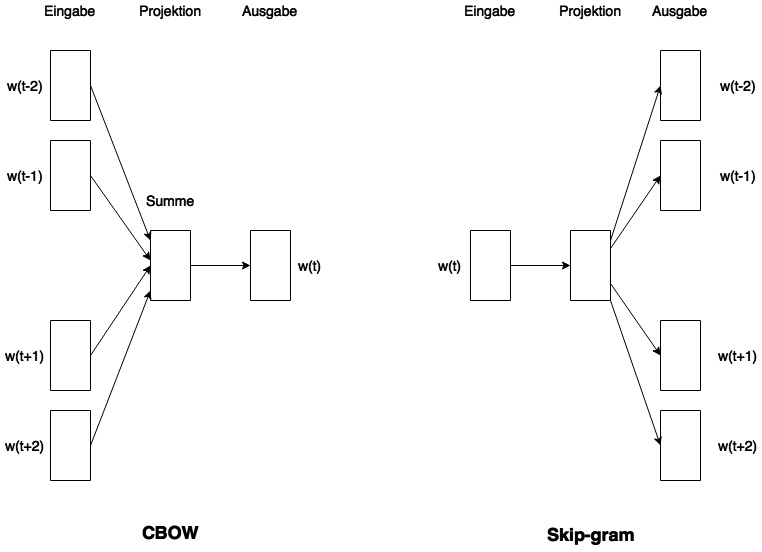
\includegraphics[scale=0.55]{CBOWvsSkip-gram.png}
  \end{center}  
  \caption{CBOW und Skip-gram im Vergleich, übersetzt nach \cite{DBLP:journals/corr/abs-1301-3781}}
  \label{cbowvsskipgram}
\end{figure}

\section*{CBOW}
Durch  Bengio et al. \cite{bengio2003neural} wurde das \textit{Feedforward Neural Net Language Model (NNLM)} beschrieben. Es ist ein neuronales Netz, mit Eingabe-, Projektions-, verdeckten- und Ausgabeschichten. Ziel des neuronalen Netzes ist es, aus N Eingabewörtern möglichst genau das darauf folgende Wort vorherzusagen.\\
Die CBOW Architektur ist ähnlich zum NNLM, allerdings wurden die verdeckten Schichten entfernt und die Projektionsschicht wird von allen Wörtern geteilt. So werden alle Wörter auf die gleiche Position projiziert (das vorherzusagende Wort). Es werden auch nicht nur vergangene Wörter, sondern auch Wörter, die dem zu vorhersagenden Wort nachstehen, beim Training benutzt. Trainingskriterium ist hier das momentane (mittlere) Wort korrekt vorherzusagen, so lange werden die Vektoren der Wortrepräsentationen ständig angepasst. Kurz gesagt, beim CBOW Algorithmus wird ein Wort aus dem Kontext vorhergesagt.



\section*{Skip-gram}
Die Architektur des Skip-grams ist ähnlich zur CBOW Architektur. Allerdings wird bei Skip-gram nicht aus dem Kontext ein Wort vorhergesagt, sondern es wird ein Bereich an Wörtern, vor und nach dem aktuellen, anhand des aktuellen Wortes vorhergesagt. Wird der Bereich, der vorhergesagt wird, vergrößert, verbessern sich die Wortvektoren, allerdings erhöht dies die Berechnungskomplexität des gesamten Models. Da weiter entferntere Wörter weniger mit dem aktuellen Wort zu tun haben, als nahestehende, wird dies in den Gewichten beim Training beachtet\citep{DBLP:journals/corr/abs-1301-3781}. Kurz gesagt, beim Skip-gram Algorithmus wird aus einem Wort der Kontext vorhergesagt.\\

Zur Skip-gram Architektur haben Mikolov et al. \citep{DBLP:journals/corr/MikolovSCCD13} eine weitere Arbeit verfasst, in der sie Methoden zur Verbesserung vorstellen, sowie die Trainingsfunktion des \textit{hierarchical softmax} erläutern und eine Alternative, das \textit{negative sampling}, vorschlagen.\\

\subsection*{Hierarchical softmax\footnote{Vergleiche \cite{DBLP:journals/corr/MikolovSCCD13} in diesem Abschnitt.}}
Ein mehr formelles Trainingsziel des Skip-gram Modells beschreiben Mikolov et al.\cite{DBLP:journals/corr/MikolovSCCD13} als die durchschnittliche log Wahrscheinlichkeit zu maximieren, gegeben einer Sequenz von Trainingsworten $w_1, w_2,...,w_T$,\\
 \begin{equation}
\frac{1}{T} \sum_{t=1}^T \sum_{-c \le j \le c, j \neq 0} \textrm{log } p(w_{t+j}|w_t) 
  \end{equation}
  wobei $c$ die Größe des Kontextes darstellt\citep{DBLP:journals/corr/MikolovSCCD13}. Die Definition der allgemeinen Softmax Funktion in Skip-gram definiert $p(w_{t+j}|w_t)$, laut Mikolov et al. \cite{DBLP:journals/corr/MikolovSCCD13}, als:
  
 \begin{equation}
p(w_O|w_I)=\frac{\exp({v'_{w_O}}^T v_{w_I}) }{\sum_{w=1}^W \exp({v'_w}^{T} v_{w_I})} 
  \end{equation}
  mit $v_w$ und $v'_w$ als \glqq Input\grqq und \glqq Output\grqq{} der Vektorrepräsentation des Wortes $w$, sowie $W$ als Anzahl der Worte im Vokabular. Weil die Wahrscheinlichkeit $p$ proportional zu $W$ ist, ist diese Definition nicht zu gebrauchen, da $W$ oft sehr groß ($10^5 - 10^7$) ist\cite{DBLP:journals/corr/MikolovSCCD13}.\\
  
Eine Annäherung an die allgemeine softmax Funktion ist die hierarchical softmax Funktion. Morin und Bengio verwendeten diese im Kontext der \textit{neuronal network language models} zuerst \cite{morin2005hierarchical}. Nach Mikolov et al. \cite{DBLP:journals/corr/MikolovSCCD13} ist der Hauptvorteil, dass anstatt $W$ Ausgabeknoten im neuronalen Netz nur ungefähr $log_2(W) $ Knoten ausgewertet werden müssen, um die Wahrscheinlichkeiten zu errechnen. Weiter beschreiben sie, dass jedes Wort $w$ durch einen geeigneten Pfad vom Wurzelknoten aus erreicht werden kann. So ist $n(w,j)$ der j-te Knoten auf dem Weg von der Wurzel zum Wort $w$ mit der Pfadlänge von $L(w)$. Daraus ergibt sich, dass $n(w,1)$ der Wurzelknoten ist und $n(w,L(w))=w$. Außerdem ist $ch(n)$ als beliebiger, aber fixer Kindknoten von $w$ definiert\citep{DBLP:journals/corr/MikolovSCCD13}. Nach Mikolov et al. \cite{DBLP:journals/corr/MikolovSCCD13} sei der Ausdruck [[x]]  gleich 1, wenn x wahr ist, andernfalls -1. Das \textit{hierarchische softmax} definiert die Wahrscheinlichkeit $p(w_O|w_I)$ wie folgt \cite{DBLP:journals/corr/MikolovSCCD13}:\\
 \begin{equation}
p(w|w_I)=  \prod_{j=1}^{L(w)-1} \sigma([[n(w,j+1) = ch(n(w,j))]]\cdot {v'_{n(w,j)}}^T v_{w_I } )
  \end{equation}
  wobei $\sigma$ die Sigmoid-Funktion $\sigma(x)=\frac{1}{1+\exp(-x)} $ darstellt.
Nach Mikolov et al. \cite{DBLP:journals/corr/MikolovSCCD13} ist belegt, dass $\sum_{w=1}^W P(w|w_I) = 1$, das impliziert, dass die Berechnungskosten von $\textrm{log } p(w_O|w_I)$ proportional zu $L(w_O)$ sind, wobei dies im Durchschnitt nicht größer als log $W$ ist. Anders als bei der allgemeinen Definition des softmax im Skip-gram, bei der jedem Wort $w$ zwei Darstellungen $v_w$ und $v'_w$ , laut Mikolov et al. \citep{DBLP:journals/corr/MikolovSCCD13}, zugeordnet werden, wird bei der Definition des hierarchical softmax jedem Wort $w$ eine Darstellung  $v_w$ und jedem inneren Knoten $n$ des Binärbaumes je eine Darstellung $v'_n$ zugeordnet.
Mikolov et al. \cite{DBLP:journals/corr/MikolovSCCD13} erklären, dass die Struktur des Baumes, der beim hierarchical softmax benutzt wird, einen großen Einfluss auf die Performanz hat. Sie verwenden einen Huffman Binärbaum, dieser ist so aufgebaut, dass häufig genutzte Worte kurze Kodierungen haben, was sich positiv auf das Trainingstempo auswirkt.\\


\subsection*{Negative sampling\footnote{Vergleiche \cite{DBLP:journals/corr/MikolovSCCD13} in diesem Abschnitt.}}
Als Alternative zur hierarchical softmax Funktion kann \textit{Noise Contrastive Estimation(NCE)} benutzt werden \cite{DBLP:journals/corr/MikolovSCCD13}. Die NCE wurde zuerst von Gutmann und Hyvarinen \cite{gutmann2012noise} beschrieben und durch Mnih und Teh \cite{mnih2012fast} im Bereich der Sprachmodellierung verwendet. Nach Mikolov et al. \cite{DBLP:journals/corr/MikolovSCCD13} sieht die NCE es für notwendig, dass ein gutes Modell Daten von Rauschen unterscheiden kann. Mikolov et al. \cite{DBLP:journals/corr/MikolovSCCD13} erläutern, dass die NCE zur Maximierung der log Wahrscheinlichkeit der softmax Funktion dienen kann, wobei sich aber das Skip-gram Modell nur mit dem Lernen von qualitativ hochwertigen Vektordarstellungen beschäftigt. Deshalb haben Mikolov et al. \cite{DBLP:journals/corr/MikolovSCCD13}, mit der Voraussetzung, dass bei der Vektordarstellung die Qualität erhalten bleibt, das \textit{Negative sampling} wie folgt definiert:\\
\begin{equation}
\textrm{log }   \sigma({v'_{w_O}}^Tv_{w_I}) + \sum_{i=1}^k \mathbb{E}_{{w_i}\sim P_n(w)}\left[\textrm{log }\sigma({-v'_{w_i}}^Tv_{w_I})\right]
\end{equation}
Mit diesem Term wird dann jeder $\textrm{log }P(w_O|w_I)$ Term im Skip-gram ersetzt. Ziel ist es, das Zielwort $w_O$ aus der Rauschverteilung $P_n(w)$ mittels logistischer Regression zu erkennen\citep{DBLP:journals/corr/MikolovSCCD13}. Bei der Regression gibt es $k$ Negativbeispiele, wobei nach Experimenten von Mikolov et al. \citep{DBLP:journals/corr/MikolovSCCD13}, $k$ zwischen 5-20 in kleineren Trainingssets und zwischen 2-5 bei großen Trainingssets liegen sollte. Mikolov et al. \citep{DBLP:journals/corr/MikolovSCCD13} fanden auch durch Experimente eine optimale Rauschverteilung für $P_n(w)$ und dass die Unigramverteilung $U(w)$ um $3/4$ potenziert (z.B. ${U(w)}^{3/4} / Z)$, die Unigram- und Uniformverteilung weit übertreffen.\\
Der Hauptunterschied zwischen Negative sampling und NCE ist nach Mikolov et al. \citep{DBLP:journals/corr/MikolovSCCD13}, dass bei der NCE sowohl die Stichprobe, als auch die numerische Wahrscheinlichkeit der Rauschverteilung gebraucht wird. Hingegen braucht Negative sampling nur die Stichproben. Sowie, dass NCE die log Wahrscheinlichkeit des softmax durchschnittlich maximiert, was aber nicht wichtig für diese Anwendung ist\citep{DBLP:journals/corr/MikolovSCCD13}.\\

Kurz gesagt, unterscheidet sich das negative sampling zum hierarchical softmax insofern, dass nicht die Ähnlichkeiten zu anderen Worten berechnet werden, sondern es wird davon ausgegangen, dass zufällig ausgewählte Worte mit einer hohen Wahrscheinlichkeit unähnlich, dem zu testenden Wort, sind.\\
	\vspace{1em}\\
Zum Training mit diesen Funktionen können folgende Parameter verwendet werden:\\

\textbf{size}
	\vspace{1em}\\
	Mit dem Parameter \textit{size} wird die Anzahl der Dimensionen der Wortvektoren eingestellt. In einem n-dimensionalen Vektorraum nimmt n den Wert von \textit{size} an. In \citep{DBLP:journals/corr/abs-1301-3781} werden bei den Beispielen Werte zwischen 50 und 1000 für \textit{size} verwendet.\\	
	
	\textbf{window}
	\vspace{1em}\\
	\textit{window} ist der maximale Abstand zwischen benachbarten Worten, innerhalb eines Satzes, die zur Berechnung der Wordvektoren betrachtet werden ($\widehat{=}$ Kontext). Auf der Google Code Seite von Word2Vec\footnote{https://code.google.com/p/word2vec/, abgerufen am 26.07.2015} wird eine \textit{window} Größe bei der Skip-gram Architektur von ungefähr zehn, bei CBOW von ungefähr fünf vorgeschlagen.\\
	
	\textbf{min\_count}
	\vspace{1em}\\
	Der Parameter \textit{min\_count} gibt an, wie oft ein Wort in den Testdaten mindestens vorkommen muss, um in das Wörterbuch aufgenommen zu werden. In der Gensim-Implementierung von Word2Vec\footnote{https://radimrehurek.com/gensim/, abgerufen am 24.06.2015} wird ein voreingestellter Wert von fünf verwendet.\\
	
	\textbf{negative}
	\vspace{1em}\\
	Dieser Parameter wird nur benötigt, wenn als Lernalgorithmus negative sampling verwendet wird. Er gibt an, wie viele zufällig ausgewählten Worte beim Test auf Ähnlichkeit verwendet werden sollen. Im Artikel von Mikolov et al. \citep{DBLP:journals/corr/MikolovSCCD13} wird für diesen Wert bei kleinen Trainingskorpora ein Wert aus dem Bereich zwischen 5 und 20 vorgeschlagen, für große Trainingskorpora zwischen 2 und 5.\\


\section*{Unterschiedliche Arten von Ähnlichkeiten}
Die gelernten Wortrepräsentationen sind erstaunlicherweise sehr gut im Erkennen von syntaktischen und semantischen Regelmäßigkeiten in natürlicher Sprache und diese bedeutungsvollen Beziehungen werden in einer sehr einfachen Art und Weise erfasst\cite{DBLP:conf/naacl/MikolovYZ13}. Es kann festgestellt werden, dass \textit{groß} zu \textit{größer} die gleiche Beziehung hat, wie \textit{klein} zu \textit{kleiner}\citep{DBLP:journals/corr/abs-1301-3781}. Dadurch können Fragen in der Art \glqq Welches Wort ist ähnlich zu \textit{klein}, in der Form in der \textit{am größten} zu \textit{groß} ähnlich ist?\grqq an das Modell gestellt werden. Um solche Fragen beantworten zu können, reicht es aus, einfache algebraische Operationen auf den Vektordarstellungen der Wörter auszuführen\citep{DBLP:journals/corr/abs-1301-3781}. So muss, um das Wort zu finden, welches ähnlich zu \textit{klein} im gleichen Sinn wie \textit{am größten} zu \textit{groß} ist, folgender Vektor errechnet werden $X = vector(\textrm{\glqq am größten\grqq}) - vector(\textrm{\glqq groß\grqq}) + vector(\textrm{\glqq klein\grqq})$, dann wird der Vektorraum abgesucht um das nächste Wort dieses Vektors $X$ zu finden\citep{DBLP:journals/corr/abs-1301-3781}. Der Abstand wird mit der Kosinusähnlichkeit gemessen. Das dann erhaltene Wort wird als Lösung für die Frage verwendet. Jede solche Ähnlichkeit wird mit einem beziehungsspezifischen Offsetvektor charakterisiert\citep{DBLP:conf/naacl/MikolovYZ13}, so sind Wortpaare, die die gleiche Art von Ähnlichkeit haben, durch den gleichen Offsetvektor getrennt. In Figur \ref{fig:offsetvectors} ist dies veranschaulicht. Dadurch, dass jede Beziehung ihren eigenen Offsetvektor hat, erlaubt es das Modell, dass die einzelnen Worte viele unterschiedliche Beziehungen haben können.\\



\begin{figure}[h]
  \begin{center}
	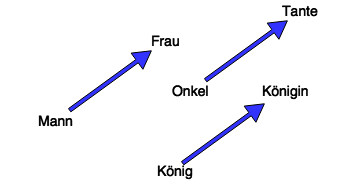
\includegraphics[scale=0.65]{OffsetVector2.png}
  \end{center}  
  \caption{Ähnlichkeiten von Worten, als Offsetvektoren dargestellt. Nach Figur 2 in \citep{DBLP:conf/naacl/MikolovYZ13}.}
  \label{fig:offsetvectors}
\end{figure}

Wortvektoren, die solche semantische Ähnlichkeiten darstellen können, könnten auch zur Verbesserung in vielen bereits existierenden NLP Anwendungen, wie maschinelles Übersetzen, Informationsgewinnung oder Systeme zur Fragebeantwortung, verwendet werden\citep{DBLP:journals/corr/abs-1301-3781}.\\



%Allgemeines zu Word2Vec,\\
 %Vergleich zu anderen\\
  %syntaktische und semantische Ähnlichkeiten werden mit word2vec abgebildet(distributet... - paper)\\
  %Vektoraddition, -subtraktion (http://www.aclweb.org/anthology/N13-1090)\\
  
\iffalse

Maucher:
mit Word2Vec möchte man ja u.a. Wörter finden, die semantisch irgendwie zusammenhängen. Dafür gab es vor Word2Vec schon andere statistische Standardmethoden wie LSI oder NNMF. Der wesentliche Unterschied ist, dass letztgenannte Verfahren Wörter dann als semantisch korreliert finden, wenn Sie in vielen Dokumenten gemeinsam vorkommen.
 Word2Vec aber erkennt Wörter dann als semantisch korreliert, wenn sie häufig im gleichen Kontext vorkommen. 
 Das ist eine ganz andere Strategie. 
 Und mit dieser neuen Strategie kommt man in vielen Anwendungen deutlich weiter als mit den herkömmlichen Methoden.\\




Old:
In Word2Vec Modellen werden Worte als Vektoren dargestellt. Hier wird mittels \textit{distributed representation}ein n-dimensionaler Vektorraum erzeugt, in dem jedes Wort aus den Trainingsdaten durch einen Vektor dargestellt wird \cite{DBLP:journals/corr/abs-1301-3781}. \\
Als nächster Schritt werden die Vektoren in ein neuronales Netz gegeben und dort mittels eines Lernalgorithmus so verändert, dass Worte mit ähnlicher Bedeutung ähnliche Vektoren haben. Die Ähnlichkeit zwischen zwei Worten kann berechnet werden, indem die Kosinusähnlichkeit zwischen den Vektordarstellungen der beiden Worte gebildet wird.\\


Die Berechnung der Wortvektoren kann mit neuronalen Netzen unterschiedlicher Architektur erreicht werden, \textit{CBOW} oder \textit{Skip-gram}. Des weiteren stehen unterschiedliche Lernalgorithmen für die neuronalen Netze zur Verfügung, \textit{hierarchical softmax}  und \textit{negative sampling}.\\
Beim Training können unterschiedliche Parameter eingestellt werden.\\

\fi


\iffalse
	\section{Hierarchical softmax}
	 the hierarchical softmax first introduced by Bengio et al[16] and
later evaluated in a paper by Morin and Bengio[17].q2


	Eine Annäherung an das allgemeine softmax ist das hierarchical softmax \citep{DBLP:journals/corr/MikolovSCCD13}. Der Hauptvorteil ist, dass anstatt W Ausgabeknoten im neuronalen Netz nur ungefähr $log_2(W) $ Knoten ausgewertet werden müssen um die Wahrscheinlichkeiten zu errechnen. \\
	Bei diesem Lernalgorithmus wird das Wörterbuch als Huffman Binärbaum dargestellt. Dies hat den weiteren Vorteil, dass häufig genutzte Worte kurze Kodierungen haben, was sich auf das Trainingstempo positiv auswirkt.\\

	\section{Negative sampling}
	\label{sec:negativeSampling}
	Alternativ zum hierarchical softmax kann das negative sampling als Lernalgorithmus für das neuronale Netz verwendet werden \citep{DBLP:journals/corr/MikolovSCCD13}.\\
	Das negative sampling unterscheidet sich zum hierarchical softmax insofern, dass nicht die Ähnlichkeiten zu anderen Worten berechnet werden, sondern es wird davon ausgegangen, dass zufällig ausgewählte Worte mit einer hohen Wahrscheinlichkeit unähnlich, dem zu testenden Wort, sind. Wie viele solcher zufällig ausgewählter Worte benutzt werden sollen kann mit dem Parameter \textit{negative} angegeben werden.\\
	
	\fi
	
	
	

	
	
\newpage
\chapter{Wikipedia-Korpus}
Im Folgenden Kapitel werden die in der Arbeit verwendeten Korpora erläutert und die im Word2Vec Modell benutzten Parameter begründet. Des Weiteren werden die benutzten Testdaten vorgestellt.
\iffalse
	Kompletter Wikikorpus: \\
	8392453 Artikel\\
	wordcount: 2919802692\\
	sentencecount: 242144317\\
	
	
	Techkorpus:\\
	187144 Artikel (2,2%)\\
	wordcount: 9866096 (0,34%)\\
	sentencecount: 3166065 (1,3%)\\
\fi
	\section{Gesamtkorpus}
	\label{sec:Gesamtkorpus}
	Da sich die Qualität  der Wortvektoren im Word2Vec Modell wesentlich mit der Menge an Trainingsdaten erhöht\citep{DBLP:journals/corr/abs-1301-3781}, werden möglichst große Textkorpora bevorzugt. Auf der Google Code Seite von Word2Vec\footnote{https://code.google.com/p/word2vec/, abgerufen am 29.06.2015}, werden für Forschungszwecke einige Beispiele für online verfügbare große Korpora genannt, dazu zählt unter anderem auch der neueste Wikipedia Auszug\footnote{http://dumps.wikimedia.org/enwiki/latest/enwiki-latest-pages-articles.xml.bz2, abgerufen am 29.06.2015}.\\
	Da in dieser Arbeit ein allgemeiner und ein domänenspezifischer Korpus als Trainingsdaten für das Word2Vec Modell verglichen werden, eignet sich der Wikipedia Korpus besonders gut. \\
	Wie in \ref{sec:Vorverarbeitung} beschrieben, müssen die Daten erst einer Säuberung unterzogen werden, um dann anschließend für das Training im Word2Vec Modell benutzt zu werden.\\
	 Der bereinigte, komplette englischsprachige Wikipedia Korpus\footnote{Dump von März 2015, http://dumps.wikimedia.org/enwiki/latest/enwiki-latest-pages-articles.xml.bz2, abgerufen am 09.04.2015} enthält 8.392.453 Artikel, 242.144.317 Sätze und 2.919.802.692 Worte.\\


Die Skip-gram Architektur verhält sich im Bezug auf syntaktische Ähnlichkeit etwas schlechter als die CBOW Architektur, allerdings ist die Skip-gram Architektur im Bezug auf semantische Ähnlichkeit der CBOW weit überlegen\citep{DBLP:journals/corr/abs-1301-3781}. Aus diesem Grund wurde die Skip-gram Architektur ausgewählt.\\
Da der \textit{hierarchical softmax} Lernalgorithmus eher für selten vorkommende Worte und der \textit{negative sampling} Lernalgorithmus eher für häufig vorkommende Worte und niedrigdimensionale Vektoren geeignet ist\footnote{https://code.google.com/p/word2vec/\#Performance, abgerufen am 01.07.2015}, wurde der  \textit{hierarchical softmax} Lernalgorithmus gewählt, da das Modell (wie im Folgenden gezeigt wird), eine hohe Dimension an Vektoren hat und auf technologiespezifische Daten getestet werden soll (siehe \ref{sec:Testdaten} Testdaten).\\


Um die optimalen Parameter für das Training des Modells herauszufinden, wurde ein kleinerer Wikipedia Auszug\footnote{http://mattmahoney.net/dc/enwik9.zip, abgerufen am 30.06.2015, beinhaltet die ersten 1 Milliarde Zeichen des Gesamtkorpus} als Trainingsdaten benutzt und mit unterschiedlichen Parametern wurden mehrere Modelle gelernt und evaluiert (siehe Tabelle \ref{tab:VergleichParameter}).\\
Die Word2Vec-Klasse in der Gensim-Implementierung beinhaltet eine Evaluationsfunktion\footnote{\textit{gensim.models.word2vec.Word2Vec.accuracy(FILENAME)}}, die die Accuracy des Models berechnet. Die Funktion erwartet einen Dateinamen einer Datei, in der jede Zeile ein 4-Tupel ist und die einzelnen Abschnitte mit \glqq : SECTION NAME\grqq{} unterteilt sind. Ein solches 4-Tupel besteht aus zwei Wortpaaren, deren Worte die gleiche Beziehung untereinander haben, zum Beispiel \glqq Athens Greece Berlin Germany\grqq , hier stellen beide Wortpaare die Beziehung zwischen einem Land und dessen Hauptstadt dar. Auf der Google Code Seite ist eine solche Datei als Beispiel vorhanden\footnote{https://code.google.com/p/word2vec/source/browse/trunk/questions-words.txt, abgerufen am 29.06.2015}. In diesem Beispiel sind 14 Kategorien\footnote{\textit{capital-common-countries, capital-world, currency, city-in-state, family, gram1-adjective-to-adverb, gram2-opposite, gram3-comparative, gram4-superlative, gram5-present-participle, gram6-nationality-adjective, gram7-past-tense, gram8-plural, gram9-plural-verbs}} mit insgesamt 19544 4-Tupel aufgelistet.\\
Das Word2Vec Modell stellt eine Funktion bereit, \textit{most\_similar(positive=[], negative=[], topn=N)}, bei der die Vektoren der Wörter im Array \textit{positive} aufaddiert und die Vektoren der Wörter in \textit{negative} davon subtrahiert werden. Die Funktion liefert die \textit{N} Wörter zurück, deren Vektordarstellungen eine maximale Kosinusähnlichkeit mit dem Ergebnis der Vektoraddition und -subtraktion haben. Diese Funktion wird auch in der Evaluationsfunktion benutzt, indem die ersten drei Wörter des 4-Tupels in \textit{positive} und \textit{negative} eingeteilt werden\footnote{\textit{most\_similar(positive=[\grq Greece\grq,\grq Berlin\grq], negative=[\grq Athens \grq], topn=1)}}, wird das vierte Wort, hier \glqq Germany\grqq, korrekt vom Model vorhergesagt, wird dieser Testdatensatz als erfolgreich gezählt. Sollten Wörter nicht im Modell dargestellt sein, wirkt sich dies nicht negativ auf die Accuracy aus, denn die Gesamtaccuracy eines Modells wird als Verhältnis, zwischen der Anzahl der richtig vorhergesagten Wörter und der Anzahl der Testdatensätze, bei denen alle Wörter eine Vektordarstellung im Modell haben, dargestellt. In der Tabelle \ref{tab:VergleichParameter} werden die unterschiedlichen Parameter\footnote{Auf der Google Code Seite von Word2Vec wird eine window size bei der Skip-gram Architektur von 10 vorgeschlagen, somit wird sie hier nicht verändert.} und die erreichte Gesamtaccuracy dargestellt. In diesem Modell waren nur bei 13144 der 19544 4-Tupel alle Wörter als Vektordarstellungen im Modell vorhanden.


\begin{table}[h]
\label{tab:VergleichParameter}
\caption{Vergleich Parameter}
\begin{center}
\begin{tabular}{l|l|l|l}
\textbf{Size} & \textbf{Window} & \textbf{Min\_count} & \textbf{Gesamtaccuracy}\\
\hline	
400 & 10 &  5 & 53,5\% (7027/13144)\\
400 & 10 & 10 & 52,5\% (6905/13144)\\
300 & 10 &  5 & 52,5\% (6860/13144)\\
300 & 10 & 10 & 52,9\% (6951/13144)\\
200 & 10 &  5 & 50,5\% (6632/13144)\\
200 & 10 & 10 & 50,5\% (6636/13144)\\
100 & 10 &  5 & 42,0\% (5517/13144)\\
100 & 10 & 10 & 41,3\% (5431/13144)\\

\end{tabular}
\end{center}
\end{table}

Auf dem kleineren Wikipedia Korpus erzielte das Modell mit den Parametern 
\textit{size} = 400, \textit{window} = 10, \textit{min\_count} = 5
 die beste Gesamtaccuracy mit 53,5\%. Diese Parameter wurden auf das Gesamtmodell übertragen. Die Trainingszeit beträgt bei diesen Parametern 10,5h\footnote{Leistungsdaten: PC mit 32 GB RAM, i7-3770 Quadcore bei 3,4 GHz} beim Gesamtmodell. Nachdem ein kleinerer Fehler im Reiningungsskript aufgetretetn war\footnote{Unbekannte Zeichen wurden mit einem Leerzeichen ersetzt, anstatt gelöscht zu werden, somit entstanden Wortfragmente als eigene Worte.}, musste das komplette Modell nochmals gelernt werden. Hier fiel dann die Entscheidung, andere Parameter zu benutzen und die \textit{window} Größe auf 300 zu reduzieren, da dies die Accuracy nur sehr gering verändert und sich die Trainingszeit auf 7,7h verkürzte. Dies zahlte sich im Laufe der Arbeit aus, da sich das Perl-Reinigungsskript ein paar Mal geringfügig änderte um so kleinere Fehler aus dem Korpus zu entfernen.\\


	
	\section{Teilkorpus}
	\label{sec:Teilkorpus}	
	Der zweite Korpus ist ein Teilkorpus des Gesamtkorpus, bestehend aus Technologieartikeln. Um diesen Korpus zu erstellen, muss der Gesamtkorpus, wie in \ref{sec:Vorverarbeitung} beschrieben, zuerst in die einzelnen Wikipediaartikel unterteilt werden. Diese Artikel werden dann mithilfe eines NBC klassifiziert. Ein NBC basiert auf dem Prinzip des überwachten Lernens. Hierzu müssen vor dem Training von Hand ausgewählte Artikel\footnote{Siehe Anhang CD} in die fünf zu klassifizierenden Themenbereiche\footnote{tech, entertainment, sport, science, politic} eingeteilt werden. In jeder Kategorie wurden gleich viele Artikel ausgewählt, somit entsteht kein Ungleichgewicht beim Training. Es wurden je Kategorie 100 Artikel verwendet. Mit diesen Daten kann der NBC dann trainiert werden. Im Anschluss daran, kann der NBC für die Klassifikation der Wikipediaartikel verwendet werden. Die Artikeln, die in die Kategorie \textit{tech} eingeteilt werden, bilden dann den technologiespezifischen Teilkorpus, der als zweiter Korpus in dieser Arbeit verwendet wird.\\
	
	
	Dieser domänenspezifische Teilkorpus enthält 187.144 Artikel (2,2\% im Vergleich zum Gesamtkorpus), 9.866.096 Wörter(0,34\%) und 3.166.065 Sätze(1,3\%). Hier beträgt die Trainingszeit ca. 2 Minuten.\\
	Wird dieser Korpus mit der \textit{.accuracy()}-Methode evaluiert, erreicht er eine Gesamtaccuracy von nur 7,0\% (490/6968). Das hat den Grund, dass die Testfragen von allgemeiner Art sind und diese Beziehungen in einem reinen Technologiekorpus sehr selten bis gar nicht vorkommen.\\
	

	Die Wahl von anderen Daten wäre auch möglich gewesen, beispielsweise könnten Korpora aus Foren zu technologischen Themen oder Technews Internetseiten, automatisch mittels Crawling, erstellt werden. Die Verwendung des Wikipedia Teilkorpus ist jedoch zielführender, da hier die gleichen Texte in beiden Korpora vorhanden sind und somit auch die gleichen Beziehungen zwischen den einzelnen Wörtern, um so einen möglichst objektiven Vergleich zwischen den unterschiedlichen Korpora zu ermöglichen.\\
	
	
	\section{Testdaten}
Im folgenden Kapitel sollen die beiden Word2Vec Modelle, deren Trainingsdaten aus dem Gesamtkorpus, beziehungsweise dem Technologiekorpus bestehen, miteinander verglichen werden. Für diesen Vergleich werden einige Experimente durchgeführt (siehe \ref{chap:Experiment1} - \ref{chap:Experiment5}), in diesen Experimenten werden die semantischen Beziehungen zwischen Wörtern betrachtet. Um diese Experimente durchführen zu können, werden Testdaten benötigt.\\
Es wird die Annahme getroffen, dass die Testdaten aus der Domäne Technologie (oder einer Unterdomäne) stammen müssen, da das Vokabular eines Modells aus Technologieartikeln besteht und auf diesen trainiert wird und da dann eher sichergestellt ist, dass diese Wörter auch wirklich im Modell vorhanden sind und somit eine Vektordarstellung haben.\\
Um diese Annahme zu überprüfen, wurden aus den drei Domänen \textit{Medizin}, \textit{Mode/Fashion} und \textit{Technologie/Pc/Internet} je 50 Begriffe ausgewählt um zu testen, ob diese überhaupt im Technologiemodell vorhanden sind\footnote{Eine vollständige Auflistung dieser Daten ist im Anhang unter \ref{Testdatenvergleich} Testdatenvergleich zu finden.}. Die Begriffe wurden von Hand aus Wikipedia Artikeln ausgesucht, um sicherzustellen, dass diese Begriffe im Gesamtmodell eine Vektorrepräsentation haben.\\
Wird im Word2Vec Modell mit der Methode \textit{most\_similar(positive=[\grq word\grq], topn=1)} nach ähnlichen Wörtern gesucht, aber das Suchwort ist nicht im Modellvokabular vorhanden, wirft diese Methode eine \glqq KeyError\grqq -Exception. Dieses Verhalten wird bei den Tests zur Überprüfung, ob die Testbegriffe im Modellvokabular vorhanden sind, benutzt. Es wird gezählt, bei wie vielen Suchbegriffen eine solche Exception geworfen wird und diese somit nicht im Modell enthalten sind.\\

Die folgende Tabelle zeigt die Resultate der Worttests. Es sind Domäne, Gesamtanzahl an Testdaten, im Modell gefundene Testdaten und im Modell nicht gefundene Testdaten dargestellt.

\begin{table}[H]
\caption{Testdatenvergleich}
\begin{center}
\begin{tabular}{|l||l|l|l|}
\hline
Domäne 	& Gesamtanzahl 	& gefundene & nicht gefundene \\
 		&  				& Testdaten	& Testdaten \\

\hline
 Medizin & 50 & 33 & 17\\
 \hline
 Mode/Fashion & 50 & 20 & 30\\
 \hline
 Technologie/Pc/Internet & 50 & 45 & 5\\
 \hline
 
\end{tabular}
\end{center}
\end{table}


Die Resultate zeigen, dass am meisten Testdaten aus der Domäne \textit{Technologie/Pc/Internet} im Modell gefunden werden.
Somit bestätigt sich die Annahme, dass die Testdaten auch aus dieser Domäne stammen sollten. 
Die Testdaten wurden dann auf 236 Begriffe erweitert\footnote{Siehe Anhang \ref{sec:Testdaten} Testdaten.}.
	
	
\newpage
\chapter{Experimente}
\label{chap:Experimente}
In diesem Kapitel sollen die beiden unterschiedlichen Word2Vec Modelle mit ihren Trainingskorpora (Gesamtkorpus und Technologiekorpus) untersucht werden. Dies soll durch fünf Experimente realisiert werden. In allen Experimenten werden semantischen Beziehungen zwischen Wörtern untersucht. Dabei ist jedes Experiment in drei Teile aufgeteilt, Beschreibung, Durchführung und Interpretation/Ergebnis.\\
Als Grundlage für die Experimente dienen die Testdaten\footnote{Siehe \ref{sec:Testdaten} Testdaten} und die mit der Methode \textit{most\_similar()\footnote{gensim.models.word2vec.Word2Vec.most\_similar()}} gefunden fünf ähnlichsten Worte. Zum Vergleichen der ähnlichen Worte der unterschiedlichen Korpora wurde eine Datei erzeugt, in der die Testdaten und ihre fünf ähnlichsten Worte, mit den dazugehörigen Kosinusähnlichkeiten, leserlich formatiert, ausgegeben werden.\\ 

	\section{Synonymsuche durch Rekursion}
\label{chap:Experiment1}
		\subsection*{Beschreibung}
		Im ersten Experiment wird untersucht, ob es möglich ist, im Word2Vec Modell Synonyme eines Begriffs zu finden. Hierzu sollen allerdings nicht die ähnlichen Worte der Testbegriffe betrachtet werden, sondern deren ähnliche Worte. Die Suche nach ähnlichen Worten wird somit ein Mal rekursiv angewandt. Die Überlegung ist, dass durch den rekursiven Aufruf Rückbeziehungen zu den ursprünglichen Suchbegriffen und deren Synonymen entstehen. Eine Anwendung für die Synonymsuche durch Rekursion könnte ein Thesaurus-Lexikon sein.\\
		
		\subsection*{Durchführung}
		Eine Liste mit den Synonymen der Testbegriffe wird vor dem Experiment mit der Hilfe eines Webservices\footnote{Über http://thesaurus.altervista.org/, abgerufen am 20.07.2015} erstellt\footnote{Siehe Anhang CD}. Dieser Webservice liefert aber nur für 108 der insgesamt 236 Testwörter Synonyme. So wurden für dieses Experiment nur diese 108 Testwörter benutzt.\\
		Im ersten Schritt dieses Experiments müssen die ähnlichen Worte ($W_1$) der Testbegriffe, mit der Methode \textit{most\_similar()} des Word2Vec Modells, herausgefunden werden. Diese fünf Wörter ($W_1$) werden in der späteren Analyse nicht betrachtet. Im nächsten Schritt werden die fünf erhaltenen ähnlichen Wörter ($W_1$) dann als Eingabe für die \textit{most\_similar()}-Methode benutzt und liefern wieder jeweils fünf ähnliche Wörter ($W_2$) zurück. Die insgesamt 25 Begriffe werden im letzten Schritt des Experiments dann mit den Synonymen des ursprünglichen Testbegriff verglichen. Sobald einer der 25 erhaltenen Begriffe in der Liste der Synonyme des jeweiligen Testwortes enthalten ist, wird dieses Wort als \textit{Synonym enthalten} gezählt.\\
		Die nachfolgende Tabelle \ref{tab:experiment1} listet die Resultate dieses Experiments auf. Es sind die Gesamtanzahl der Testwörter, die Anzahl an Testwörter, bei denen Synonyme gefunden wurden und die Anzahl der Testwörter, bei denen keine Synonyme gefunden wurden, sowie die Anzahl der Worte, die nicht im jeweiligen Modell enthalten sind, abgebildet.
		
		

		
		
\begin{table}[H]
\caption{Experiment 1: Synonyme durch Rekursion}
\label{tab:experiment1}
\begin{center}
\begin{tabular}{|l||l|l|l|l|}
\hline
\textbf{Modell} & \textbf{Gesamtanzahl}	&\textbf{Synonyme} & \textbf{Synonyme}  & \textbf{Worte nicht}  \\
 &			& \textbf{nicht enthalten} & \textbf{enthalten} & \textbf{im Korpus}  \\

\hline
 Gesamt & 108 & 96 & 12 & 0 \\
 \hline
 Technologie & 108 & 101 & 2 & 5 \\
 \hline
 
\end{tabular}
\end{center}
\end{table}
		

\begin{table}[H]
\caption{Alle gefundenen Synonyme durch Rekursion}
\label{tab:bspsynoyme}
\begin{center}
\begin{tabular}{|l||l|l|l|l|}
\hline
\textbf{Suchbegriff} & \textbf{Modell} & \textbf{Synonym}   \\

\hline
 engineering & Technologie & discipline \\
 \hline	
 power	& Technologie	& supply	\\
 \hline
 \hline
auto & Gesamt & automobile\\
\hline
automobile & Gesamt & car\\
\hline
cyberwar & Gesamt & cyberterrorism\\
\hline
encryption & Gesamt & cryptography\\
\hline
google & Gesamt & search\\
\hline
linux & Gesamt & unix\\
\hline
mouse & Gesamt & rodent\\
\hline
processor & Gesamt & cpu\\
\hline
sun & Gesamt & star\\
\hline
telecom & Gesamt & telecommunication\\
\hline
television & Gesamt & tv\\
\hline
wifi & Gesamt & wlan\\
 	\hline
 
\end{tabular}
\end{center}
\end{table}
		
 In der Tabelle \ref{tab:bspsynoyme} sind alle gefundenen Synonyme und die dazugehörigen Testwörter, sowie der Korpus in dem sie auftreten, aufgelistet.
		
		\subsection*{Interpretation/Ergebnis}
		Wie aus den Daten hervorgeht, werden im Gesamtmodell nur bei zwölf, im Technologiemodell nur bei zwei Testbegriffen Synonyme gefunden.
		Ein Grund, der die geringe Anzahl an Synonymen erklären könnte, könnte mit der räumlichen Darstellung der Worte im Word2Vec Modell zusammenhängen. Die ähnlichen Worte ($W_1$) eines Suchbegriffs ($O$) haben einen minimalen räumlichen Abstand zum Suchbegriff (O). 
		Die durch die Rekursion erhaltenen ähnlichen Worte ($W_2$) der ähnlichen Worte ($W_1$), haben wieder einen minimalen räumlichen Abstand (zu $W_1$), allerdings ist der Abstand vom ursprünglichen Suchbegriff ($O$) zu den in $W_2$ enthaltenen Wörter größer als zu den Worten aus $W_1$, denn sonst wären sie schon in der Menge $W_1$ enthalten. Also sind diese Wörter noch weiter vom ursprünglichen Suchbegriffs ($O$) entfernt und somit unähnlicher. Somit ist das Finden von Synonymen durch Rekursion im Word2Vec Modell nicht zielführend.\\
		Des Weiteren kann das Ergebnis mit den verwendeten Synonymen zusammen hängen. Werden ausführlichere Listen mit Synonymen verwendet, sollte sich damit auch die Anzahl der vom Modell gefundenen Synonyme erhöhen.\\
		
		
	
	\section{Konkretisierungen}
		\subsection*{Beschreibung}
		In diesem Experiment soll hauptsächlich das domänenspezifischen Technologiemodell untersucht werden. Es wird untersucht, ob die ähnlichen Wörter der Testdaten eine Konkretisierung des jeweiligen Suchbegriffs darstellen.	Dies ist gerade bei mehrdeutigen Wörtern interessant, da dann eine Sinnrichtung in den ähnlichen Wörtern dominant vertreten sein könnte und somit klar ist, in welchem Kontext das mehrdeutige Wort in dieser Domäne gemeint ist. Es wird vermutet, dass im Technologiemodell die Konkretisierungen stärker vorhanden sind als im allgemeinen Modell. In diesem Experiment werden wieder alle 236 Testdaten verwendet.\\
		
				Es wird definiert, dass von einer Konkretisierung gesprochen werden kann, wenn das ähnliche Wort eine genauere Bedeutung des Suchbegriffs darstellt (z.B. wird \textit{Wissenschaftler} durch \textit{Physiker} konkretisiert). In der Abbildung \ref{pic:Konkretisierung} sind die Abstraktionsbeziehungen zwischen Wörtern als Baumdiagramm dargestellt. Gelb markiert ist der aktuelle Suchbegriff, alle Kindknoten des Suchbegriffs sind grün markiert, hier kann von einer Konkretisierung des Suchbegriffs gesprochen werden. Rot markiert sind alle anderen Knoten, hier kann nicht von einer Verallgemeinerung gesprochen werden. Zur vereinfachten Darstellung ist die Abbildung in 2D und mit einer einfachen Struktur ausgewählt, in komplizierteren Beispielen, unter anderem auch mit mehrdeutigen Begriffen, muss überlegt werden ob eine solche Darstellung überhaupt noch möglich ist.\\
		
\begin{figure}[h]
  \begin{center}
	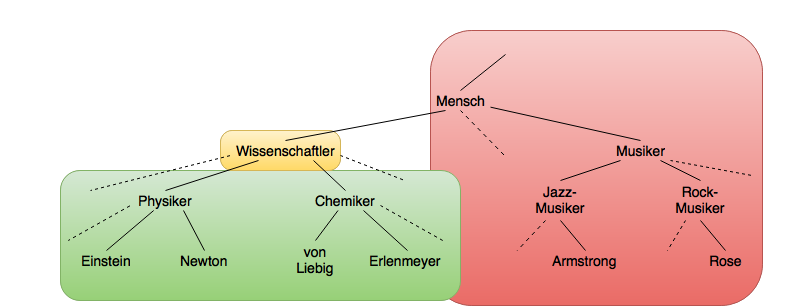
\includegraphics[scale=0.55]{Konkretisierung_Baum2.png}
  \end{center}  
  \caption{Beispiel der Beziehungen zwischen Wörtern, im Bezug auf Konkretisierung, als Baumdiagramm dargestellt.}
  \label{pic:Konkretisierung}
\end{figure}
		
		\subsection*{Durchführung}
		Die Fragestellung bezieht sich zwar eigentlich auf das domänenspezifische Modell, allerdings wurde auch das allgemeine Modell auf diese Fragestellung hin untersucht um festzustellen, ob dieses tatsächlich ein schlechteres Verhalten bezüglich der Anzahl an gefundenen Konkretisierungen aufweist.\\
		Bei diesem Experiment werden die Testwörter mit ihren fünf ähnlichsten Wörtern verglichen. Diese Untersuchung erfolgt von Hand, da es keine Auflistungen mit Konkretisierungen von Begriffen gibt. Außerdem wäre es zu aufwändig, eine solche Liste zu erstellen, da nicht vorhersehbar ist, wie stark die Suchbegriffe konkretisiert werden und somit sehr viele Daten erzeugt werden müssten. Sollten die Modelle hinsichtlich der Konkretisierungstiefe\footnote{Damit ist gemeint ob z.B. der Begriff \textit{Auto} mit \textit{BMW, Mercedes, VW} oder aber mit \textit{X5, A-Klasse, Tuareg} konkretisiert wird.} untersucht werden, könnte das in einem zusätzlichen Experiment analysiert werden. Dann müssten solche Auflistungen mit Konkretisierungen von Begriffen erstellt werden, um das unterschiedliche Verhalten aufzuzeigen. In diesem Experiment geht es aber darum, erst einmal herauszufinden, ob überhaupt eine Konkretisierung stattfindet, unabhängig von der Konkretisierungstiefe.\\	
		 Stellen mindestens drei der fünf ähnlichen Wörter eine Konkretisierung des Suchbegriffs dar, so wird dieser Eintrag als \textit{konkretisiert} markiert. Bei diesem Experiment war das Nachschlagen von mehreren ähnlichen Worten sehr zeitintensiv, denn um beurteilen zu können, ob es sich bei diesem Wort um eine Konkretisierung des Suchbegriffs handelt, müssen die inhaltlichen Beziehungen zwischen Suchbegriff und ähnlichen Worten klar sein. Um die Bedeutungen der Worte und die inhaltlichen Beziehungen zu recherchieren, wurde Wikipedia\footnote{https://en.wikipedia.org/, abgerufen am 21.07.2015} und Google\footnote{https://www.google.de/, abgerufen am 21.07.2015} benutzt.\\
		
		In der folgenden Tabelle sind die Gesamtanzahl der Testwörter, die Anzahl der Suchbegriffe, die mit \textit{konkretisiert} markiert wurden, die Anzahl der Suchbegriffe,  die nicht mit \textit{konkretisiert} markiert wurden, sowie die Anzahl der nicht im Modell enthaltenen Worte, dargestellt. Die Daten sind nach Modellen getrennt aufgelistet. Des Weiteren sind einige Beispiele in Tabelle \ref{tab:BspKonkretisierung} aufgelistet. Diese Tabelle enthält neben den Suchbegriffen, Modell und den gefundenen konkretisierten ähnlichen Worten auch die Kosinusähnlichkeiten zu den Suchbegriffen.
		
\begin{table}[H]
\caption{Experiment 2: Konkretisierung}
\begin{center}
\begin{tabular}{|l||l|l|l|l|}
\hline
\textbf{Modell} & \textbf{Gesamtzahl}& \textbf{ähnliche Worte} & \textbf{ähnliche Worte}  & \textbf{Wort nicht}  \\
 & &\textbf{nicht konkretisiert} & \textbf{konkretisiert} & \textbf{im Korpus} \\

\hline
 Gesamt & 236 & 199 & 37 & 0 \\
 \hline
 Technologie & 236 & 146 & 65 & 25 \\
 \hline
 
\end{tabular}
\end{center}
\end{table}
		
		

\begin{table}[H]
\caption{Beispiele zur Konkretisierung}
\label{tab:BspKonkretisierung}
\begin{center}
\begin{tabular}{|l||l|l|l|l|}
\hline
\textbf{Suchbegriff} & \textbf{Modell} & \textbf{Konkretisierung}   \\

\hline
 apple & Technologie & iphone (Kosinusähnlichkeit: 0,587), a6x (0,579)\\
 & & ipad (0,570), a5x (0,559)\\
 \hline
 architecture	   & Gesamt & revival (0,774), neoclassical (0,677), gothic (0,667) \\
 & Technologie& armv7a (0,514), multicore (0,493), xmos (0,477) \\
\hline
 fat	& Technologie	& exfat (0,751), vfat (0,724), fat32 (0,709)	\\
 	\hline
 intel	 & Technologie& i7 (0,707), t2300 (0,702), i5 (0,666), i52450m (0,663) \\
 \hline
 photography	& Technologie& slrs(0,544), panoramic (0,543), polaroid (0,531)\\
 	\hline
 power	&	Gesamt &	electricity (0,679), surgut2 (0,637), egbin (0,627) \\
 	\hline
 
\end{tabular}
\end{center}
\end{table}
		
		
		\subsection*{Interpretation/Ergebnis}
Im Technologiemodell konkretisieren in 65 der 236 Testfälle	die ähnlichen Worte den jeweiligen Suchbegriff, im Gesamtmodell jedoch nur in 37 Fällen. Somit bestätigt sich die Annahme, dass im Gesamtmodell weniger Konkretisierungen auftreten. Dies hat den Grund, dass sich die Daten im Gesamtmodell nicht auf eine Fachrichtung beschränken wie im Technologiemodell. So werden beim Training mit Technologiedaten im Word2Vec Modell die Beziehungen beibehalten, die beim Training mit dem kompletten Wikipediakorpus durch andere, allgemeine Wörter noch weiter verändert werden. \\
Da die Anzahl der Testfälle, bei denen die ähnlichen Wörter den Testbegriff konkretisieren, nicht so hoch ist, kann daraus geschlossen werden, dass diese Begriffe und die Worte, die sie konkretisieren, nicht so häufig im gleichen Kontext in den Trainingsdaten vorhanden waren.\\
		
		
	
	\section{Verallgemeinerungen}
		\subsection*{Beschreibung}
		In diesem Experiment wird analysiert, ob die ähnlichen Worte eines Begriffs eine Verallgemeinerung dessen darstellen. Es wird außerdem untersucht, ob im allgemeinen Gesamtmodell mehr Begriffe in ihren ähnlichen Wörtern verallgemeinert werden, als im Technologiemodell. Ein Anwendungsbeispiel für die Verallgemeinerung der Suchbegriffe könnte ein Lexikon sein, bei dem die Worte mit ähnlichen Begriffen beschrieben werden. In diesem Experiment werden wieder alle 236 Testdaten verwendet.\\
		Es wird definiert, dass von einer Verallgemeinerung gesprochen werden kann, wenn das ähnliche Wort eine abstraktere Bedeutung des Suchbegriffs darstellt (z.B. wird \textit{Physiker} durch \textit{Mensch} verallgemeinert) oder das ähnliche Wort bildet einen vergleichbaren Begriff (kein Synonym) ab (z.b. kann \textit{Physiker} mit \textit{Chemiker} verallgemeinert werden). In der Abbildung \ref{pic:Verallgemeinerung} sind die Abstraktionsbeziehungen zwischen Wörtern als Baumdiagramm dargestellt. Gelb markiert ist der aktuelle Suchbegriff, Elternknoten und direkte Geschwisterknoten sind grün markiert, hier kann von einer Verallgemeinerung des Suchbegriffs gesprochen werden. Rot markiert sind die Kindknoten und weiter entfernte Knoten, hier kann nicht von einer Verallgemeinerung gesprochen werden. Zur vereinfachten Darstellung ist die Abbildung in 2D und mit einer einfachen Struktur ausgewählt, in komplizierteren Beispielen, unter anderem auch mit mehrdeutigen Begriffen, muss überlegt werden ob eine solche Darstellung überhaupt noch möglich ist.\\
		
\begin{figure}[h]
  \begin{center}
	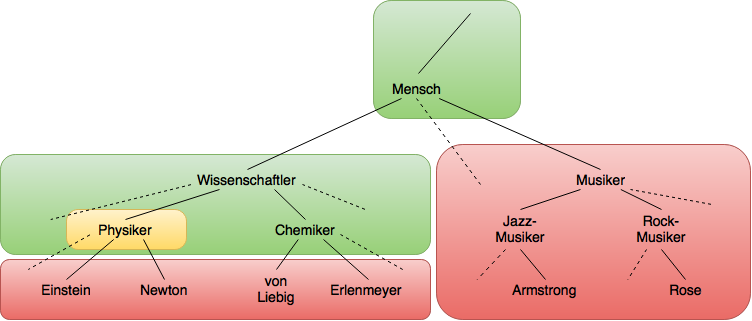
\includegraphics[scale=0.55]{Verallgemeinerung_Baum2.png}
  \end{center}  
  \caption{Beispiel der Beziehungen zwischen Wörtern, im Bezug auf Verallgemeinerung, als Baumdiagramm dargestellt.}
  \label{pic:Verallgemeinerung}
\end{figure}
		
		\subsection*{Durchführung}
		In diesem Experiment werden die Testdaten, wie im vorherigen Experiment, mit ihren fünf ähnlichsten Wörtern verglichen. Auch diese Untersuchung wird von Hand durchgeführt, denn auch hier soll, wie im vorherigen Experiment, erst einmal untersucht werden, ob Verallgemeinerungen überhaupt auftreten. In einem weiteren Experiment könnte auch hier untersucht werden, welchen Grad die Verallgemeinerungen haben\footnote{Damit ist gemeint ob \textit{Albert} mit \textit{Einstein}, \textit{Physiker}, \textit{Wissenschaftler} oder \textit{Mensch} verallgemeinert wird.}. Verallgemeinern drei der fünf ähnlichen Worte den Suchbegriff, wird dieser als \textit{verallgemeinert} markiert. 
		
		
		Wie beim vorherigen Experiment mussten viele Begriffe nachgeschlagen werden,  um die inhaltlichen Beziehungen zwischen dem Suchbegriff und den jeweiligen ähnlichen Worten beurteilen zu können.\\
		
In Tabelle \ref{tab:Experiment3} sind die Gesamtzahl der Testwörter, die Anzahl der Suchbegriffe, die mit \textit{verallgemeinert} markiert wurden, die Anzahl der Suchbegriffe,  die nicht mit \textit{verallgemeinert} markiert wurden, sowie die Anzahl der Worte, die nicht im Modell enthalten sind, aufgelistet. Die Daten sind nach Modellen getrennt aufgelistet. Die Tabelle \ref{tab:bspVerallgemeinerung} enthält einige Beispiele der gefundenen Verallgemeinerungen. Es sind neben den Suchbegriffen, Modell und den gefundenen verallgemeinerten ähnlichen Worten, auch deren Kosinusähnlichkeiten zu den Suchbegriffen.
		
\begin{table}[H]
\caption{Experiment 3: Verallgemeinerung}
\label{tab:Experiment3}
\begin{center}
\begin{tabular}{|l||l|l|l|l|}
\hline
\textbf{Modell} & \textbf{Gesamtzahl}& \textbf{ähnliche Worte} & \textbf{ähnliche Worte}  & \textbf{Wort nicht} \\
 &  & \textbf{nicht verallgemeinert} & \textbf{verallgemeinert} &\textbf{ im Korpus} \\

\hline
 Gesamt & 236 & 102 & 134 & 0  \\
 \hline
 Technologie & 236 & 144 & 67 & 25 \\
 \hline
 
\end{tabular}
\end{center}
\end{table}


		
		
\begin{table}[H]
\caption{Beispiele zur Verallgemeinerung}
\label{tab:bspVerallgemeinerung}
\begin{center}
\begin{tabular}{|l||l|l|l|l|}
\hline
\textbf{Suchbegriff} & \textbf{Modell} & \textbf{Verallgemeinerung}   \\
\hline
 apple & Gesamt & blackberry (Kosinusähnlichkeit: 0,704),\\
 	&	& raspberry (0,657), webos (0,643)\\
 \hline
 asus	   & Gesamt & netbook (0,767), lenovo (0,736), motherboards (0,714) \\
\hline
 cookies	& Gesamt& baked (0,666), cakes (0,663), muffins (0,654)\\
 	\hline
 dell	 & Gesamt & hewlettpackard (0,583), cisco (0,548), lenovo (0,515),\\
 && compaq (0,506) \\
 \hline
 limewire	& Gesamt& bittorrent (0,703), filesharing (0,702), kazaa (0,689)\\
 &&rapidshare (0,668), gnutella (0,653)\\
 	\hline
 	
 photoshop &	Technologie&	illustrator (0,781), lightroom (0,758), cs3 (0,710) \\
 	\hline
 	
 
\end{tabular}
\end{center}
\end{table}


  
		\subsection*{Interpretation/Ergebnis}
		Im Gesamtmodell weisen bei 134 Testbegriffen mindestens drei der dazugehörigen ähnlichen Worte eine Verallgemeinerung des Testwortes auf. Im Technologiemodell ist dies nur bei 67 Begriffen der Fall. Somit bestätigt sich die Vermutung, dass im Gesamtmodell mehr Verallgemeinerungen zu finden sind. Dies hängt mit der Tatsache zusammen, dass das Gesamtmodell mit Daten, die nicht auf ein spezielles Thema beschränkt sind, trainiert wurde und diese Begriffe in vielen unterschiedlichen Zusammenhängen im Trainingskorpus enthalten sind. Die allgemeineren ähnlichen Worte müssen in den Trainingsdaten also häufiger im gleichen Kontext wie die Testbegriffe vorgekommen sein, als andere Worte.\\
		
		
		
		
	
	\section{Unterschiedliche Beziehungen}
		\subsection*{Beschreibung}
		Die inhaltlichen Beziehungen zwischen Wörtern können von unterschiedlicher Art sein. So können die Wörter \textit{\textbf{Gleiches}} darstellen, beispielsweise stellen sowohl \glqq dropbox\grqq, als auch \glqq icloud\grqq{}  oder \glqq onedrive\grqq{} Cloud-Speicher dar. Außerdem können Wörter auch \textit{\textbf{Gegenteiliges}} darstellen, wie z.B. \glqq heiß\grqq{} und \glqq kalt\grqq. \textit{\textbf{Syntaktisch}} ist eine weitere Beziehungsart, wie bei \glqq Verschlüsselung\grqq{} und \glqq verschlüsseln\grqq. \glqq Automobil\grqq{} und \glqq KFZ\grqq{} haben eine \textit{\textbf{synonyme}} Beziehung untereinander. Trifft keine der bisher genannten Arten auf die Beziehung zwischen zwei Wörtern, diese haben aber trotzdem etwas miteinander zu tun, wie beispielsweise \glqq Motor\grqq{} und \glqq Benzin\grqq{}, dann stehen diese Begriffe \textit{\textbf{in Beziehung}} miteinander. Diese fünf Beziehungsarten sollen als Kategorien für dieses Experiment dienen.\\
		 Ziel dieses Experiments ist festzuhalten, ob in den beiden Modellen die Trainingsbegriffe zu ihren ähnlichen Wörtern unterschiedliche Arten von Beziehungen haben. Die Auswertung der Testbegriffe und ihrer ähnlichen Wörter erfolgt hier wieder von Hand. Sobald eine Beziehungsart in mindestens drei der fünf ähnlichen Wörter abgebildet ist, wird dieser Testbegriff mit der jeweiligen Beziehungsart markiert. Erreicht keine Art drei Vorkommen, wird dieser Begriff mit \textit{\textbf{verschiedenes}} markiert, da hier eine Art nicht eindeutig zuordenbar ist. Somit ergeben sich die sechs endgültigen, unterschiedlichen Beziehungskategorien \textit{syntaktisch, synonym, gleiches, gegenteiliges, in Beziehung} und \textit{verschiedenes}. Es werden alle 236 Testbegriffen für dieses Experiment verwendet.\\
		

		\subsection*{Durchführung}
		Für dieses Experiment werden beide Modelle untersucht, um eine Aussage zu treffen, ob sich die Beziehungsarten unterscheiden. Auch hier wird von Hand die Art, die die Beziehung zwischen den einzelnen Testbegriffen und den dazugehörigen ähnlichen Wörtern beschreibt, dem jeweiligen Testbegriff zugeordnet. \\
		In der Tabelle \ref{tab:experiment4} werden die Beziehungsarten und die Anzahl der Testbegriffe, die mit der jeweiligen Art markiert sind, nach Modelltyp getrennt, dargestellt. In der darauffolgenden Tabelle \ref{tab:bspBeziehungsarten} sind Beispiele zu den einzelnen Beziehungsarten aufgelistet. Neben der Art der Beziehungen ist der Suchbegriff, Modelltyp und die ähnlichen Worte mit den dazugehörigen Kosinusähnlichkeiten abgebildet.\\
		
		
		
\begin{table}[H]
\caption{Experiment 4: Arten von Beziehungen}
\label{tab:experiment4}
\begin{center}
\begin{tabular}{|l||l|l|}
\hline
\textbf{Beziehungsart}	& \textbf{Gesamtmodell}	&   \textbf{Technologiemodell}   \\

\hline
 syntaktisch & 0 	& 0 \\
 \hline
 gegenteilig & 0 	& 0  \\
 \hline
 gleiches & 81 	& 38  \\
 \hline
 synonym & 0 	& 0  \\
 \hline
 in Beziehung & 118 	& 126 \\
 \hline
 verschiedenes & 37	& 47 \\
 \hline
 nicht im Modell & 0  & 25  \\
 enthaltene Worte &   &\\
 \hline
 
\end{tabular}
\end{center}
\end{table}
		
		

\begin{table}[H]
\caption{Beispiele zur den verschiedenen Beziehungsarten}
\label{tab:bspBeziehungsarten}
\begin{center}
\begin{tabular}{|l||l|l|l|l|}
\hline
\textbf{Art} & \textbf{Suchbegriff} & \textbf{Modell} & \textbf{Ähnliche Worte}   \\
\hline
 gleiches &chrome	   & Gesamt & firefox (0,784), safari (0,686), ie8 (0,674) \\
   &	   & Technologie & firefox (0,733), safari (0,769), flock (0,667),\\
   &&& seamonkey (0,650) \\
\hline
 in Beziehung& browser	 & Gesamt & browsers (0,882), firefox (0,812),\\
 &&& desktop (0,755), javascript (0,751)\\
 \hline
verschiedenes& encryption	& Gesamt&  encrypted (0,833),  authentication(0,815),\\
&&&  encrypts (0,798),  decryption (0,789)\\
 	\hline
 
\end{tabular}
\end{center}
\end{table}

		
		
		
		
		
		\subsection*{Interpretation/Ergebnis}
		Wie aus Tabelle \ref{tab:experiment4} ersichtlich ist, wurden keine Testbegriffe mit \textit{synonym}, \textit{syntaktisch} oder \textit{gegenteilig} markiert. Das hängt damit zusammen, dass die Bedingung für die Markierung war, dass diese Beziehungsart in mindestens drei der fünf ähnlichen Worte vorhanden sein muss. Zwar traten diese Arten der Beziehung vereinzelt auf, aber die Bedingung konnten diese drei Arten bei keinem Testbegriff erfüllen. Meist fielen diese Begriffe in die Kategorie \textit{verschiedenes}, da auch noch andere Arten vorhanden waren, aber keine dominierte. Mit einer Anzahl von 118 im Gesamtmodell und 126 im Technologiemodell war die Beziehungsart \textit{in Beziehung} am häufigsten vorhanden. Dies kann damit erklärt werden, dass im Word2Vec Modell Wörter die in ähnlichem Kontext stehen, auch nahe in der Vektorrepräsentation zusammen stehen. Die Art \textit{gleiches} war mit 81 Markierungen im Gesamtmodell am zweithäufigsten vorhanden, auch hier liegt nahe, dass es daran liegt, dass Wörter mit gleichem Kontext eine ähnliche Vektorrepräsentation haben. Im Technologiemodell tritt diese Beziehungsart nur 38 Mal auf, was daher kommen könnte, dass dieses Modell mit weniger Daten trainiert wurde und deswegen die Anzahl an Worte, die im gleichen Kontext stehen, auch geringer ist. Im Gesamtmodell steht die Art \textit{verschiedenes} mit 37 Vorkommen an dritter Stelle, beim Technologiemodell mit 47 an zweiter. Diese Art sagt nichts über die tatsächlichen Beziehungen aus, außer dass nicht eindeutig eine Art dominant vorhanden ist. \\
		In beiden Modellen sind die vorhandenen Arten die gleichen. Das Gesamtmodell stellt verhältnismäßig mehr \textit{gleiches} als das Technologiemodell dar, das Technologiemodell jedoch mehr \textit{verschiedenes} und \textit{in Beziehung}. Der Unterschied in der Anzahl der vorkommenden Beziehungsarten ist erkennbar, allerdings ist er in den unterschiedlichen Modellen nicht sehr groß.
		
		
		
		
		
		
	
	\section{Erkennen von Mehrdeutigkeit}
	
\label{chap:Experiment5}
		\subsection*{Beschreibung}
		Das letzte Experiment beschäftigt sich mit der Mehrdeutigkeit von Worten. Es wird untersucht, ob im Gesamtmodell die ähnlichen Worte eines mehrdeutigen Suchbegriffs, dessen unterschiedliche Bedeutungen repräsentieren. Oder ob dieses Verhalten häufiger im Technologiemodell aufzufinden ist.
		Hier werden nur die 66 mehrdeutigen der insgesamt 236 Testbegriffen verwendet\footnote{Siehe Auflistung der mehrdeutigen Testworte unter \ref{sec:mehrdeutigetestbegriffe} .}. \\
		
		
		\subsection*{Durchführung}
Wie in den vorherigen Experimenten, werden in diesem Experiment die Testbegriffe und ihre fünf ähnlichen Worte von Hand analysiert. Sobald zwei der ähnlichen Wörter unterschiedliche Bedeutungen eines mehrdeutigen Testbegriffes darstellen, wird dieser Begriff als \textit{Mehrdeutigkeit erkannt} markiert. Sollte dies nicht der Fall sein, werden sie mit \textit{Mehrdeutigkeit nicht erkannt} markiert. Es werden beide Modelle untersucht.\\
In Tabelle \ref{tab:experiment51} werden die Anzahl der mehrdeutigen Testbegriffe, die Anzahl der nicht mehrdeutigen Testbegriffe und wie viele der Testbegriffe jeweils nicht im Modell vorhanden sind, nach Modelltyp getrennt, aufgelistet. Die Tabelle \ref{tab:experiment52} bezieht sich komplett auf die mehrdeutigen Testbegriffe. Hier sind die Anzahl der Testbegriffe, die mit \textit{Mehrdeutigkeit erkannt}, sowie mit \textit{Mehrdeutigkeit nicht erkannt} markiert sind und die Anzahl der mehrdeutigen Testworte, die nicht im Modell enthalten sind, dargestellt. Einige Beispiele der erkannten und nicht erkannten Mehrdeutigkeiten sind in Tabelle \ref{tab:bspMehrdeutigkeiten} aufgelistet. Neben dem Suchbegriff, Modelltyp ist auch angegeben, ob die Begriffe als mehrdeutig erkannt wurden und es sind die jeweiligen ähnlichen Worte mit ihren Kosinusähnlichkeiten aufgeführt. \\

		
		\begin{table}[h]
\caption{Experiment 5: Aufteilung mehrdeutiger Worte}
\label{tab:experiment51}
\begin{center}
\begin{tabular}{|l||l|l|}
\hline
				& \textbf{Gesamtmodell}		  & \textbf{Technologiemodell}   \\

\hline

 nicht mehrdeutig & 170 & 170\\
 
davon Worte nicht im Korpus& 0   	& 24   \\
 \hline
 mehrdeutig & 66   	& 66 \\
davon Worte nicht im Korpus& 0   	& 1   \\
 \hline

\end{tabular}
\end{center}
\end{table}
		\begin{table}[h]
\caption{Experiment 5: Erkennen von mehrdeutigen Wörtern}
\label{tab:experiment52}
\begin{center}
\begin{tabular}{|l||l|l|}
\hline

	& \textbf{Gesamtmodell}	 	& \textbf{Technologiemodell}   \\

 \hline
 nicht erkannt & 59 &   58 \\
 \hline
 erkannt & 7 & 7  \\
\hline
 Wort nicht im Korpus & 0 & 1 \\
 \hline
\end{tabular}
\end{center}
\end{table}
		
\begin{table}[H]
\caption{Beispiele zur Erkennung von Mehrdeutigkeiten}
\label{tab:bspMehrdeutigkeiten}
\begin{center}
\begin{tabular}{|l||l|l|l|l|}
\hline
\textbf{Suchbegriff} & \textbf{Modell} & \textbf{Erkannt} & \textbf{Ähnliche Worte}   \\
\hline
 trojan & Gesamt & ja &rsplug (Kosinusähnlichkeit: 0,472), athena (0,462)\\
 &	&	& bundestrojaner (0,496), centaurs (0,475) \\
 &  Technologie & ja & horse (0,586), malware (0,560), zinaps (0,476)\\
 \hline
 
raspberry& Gesamt& nein & apple (0,657), apricot (0,629), \\
&&&blackcurrant (0,586),  \\
&Technologie & nein & pi (0,677), cubieboard (0,524), trimeslice (0,519)\\
\hline
 
\end{tabular}
\end{center}
\end{table}
		
		
		\subsection*{Interpretation/Ergebnis}
		


		
		Im beiden Modellen werden von den 66 mehrdeutigen Testbegriffen nur sieben erkannt. Jedoch sind dies 13 unterschiedliche Testbegriffe, denn die Modelle erkennen immer bei unterschiedlichen Begriffen die Mehrdeutigkeit und nur beim Begriff \textit{trojan} erkennen beide Modelle die Mehrdeutigkeit. Ein mehrdeutiger Testbegriff kommt im Technologiemodell gar nicht vor und 59 im Gesamtmodell beziehungsweise 58 im Technologiemodell mehrdeutige Begriffe werden nicht erkannt. Die sehr geringe Anzahl an erkannten Mehrdeutigkeiten kann auch damit zusammen hängen, dass diese Begriffe in den unterschiedlichen Bedeutungen oft sehr unterschiedliche Dinge beschreiben und somit eher selten im gleichen Kontext in den Trainingsdaten vorkommen. Und da Word2Vec die Ähnlichkeiten über den gleichen Kontext bildet, kann die Mehrdeutigkeit schlecht damit abgebildet werden.\\
Allerdings werden bei 35 Testbegriffen in den unterschiedlichen Modellen je eine unterschiedliche Bedeutung der mehrdeutigen Begriffe in den ähnlichen Worten dargestellt. Siehe dazu Tabelle \ref{tab:bspJeEinModellMehrdeutig}, dort sind einige Beispiele aufgelistet. Dargestellt sind die Testbegriffe, Modelltyp und die erhaltenen ähnlichen Worte mit Kosinusähnlichkeiten.\\
		
		\begin{table}[H]
\caption{Beispiele Mehrdeutigkeiten in unterschiedlichen Modellen}
\label{tab:bspJeEinModellMehrdeutig}
\begin{center}
\begin{tabular}{|l||l|l|l|l|}
\hline
\textbf{Suchbegriff} & \textbf{Modell} & \textbf{Ähnliche Worte}   \\
\hline

 
architecture & Gesamt		&  revival (Kosinusähnlichkeit: 0,774), neoclassical (0,677), \\
&				&  gothic (0,666),  \\
&Technologie 	&  armv7a (0,514), multicore (0,494), xmos (0,477)\\
\hline
fat & Gesamt		&  calories (0,615), milk (0,598), fatfree (0,595) \\
&Technologie 	&  ntfs (0,780), exfat(0,751), fat32 (0,709) \\
\hline
 keyboard & Gesamt		&  synthesizer (0,769), accordion (0,768), guitar (0,752)\\
&Technologie 	&  qwerty (0,672), mouse (0,667), keypad(0,641)\\
\hline
pi  & Gesamt	 &  theta (0,754), tau (0,729), rho (0,729), mu (0,695)\\
 &  Technologie  &  raspberry (0,677), cubieboard (0,478), iyonix (0,455)\\
 \hline
 ps2 & Gesamt		&  ps3 (0,795), gamecube(0,764), n64 (0,756), snes (0,748)\\

&Technologie 	&  keyboardmouse (0,764), centronics (0,676), rs232 (0,664)\\
\hline
 windows & Gesamt		&  sunhoods (0,745), sixoverone (0,743), \\
&				&  nineovernine (0,736), sixoversix (0,721)  \\
&Technologie 	&  vistawindows (0,699), vista (0,683), xp (0,656)\\
\hline
\end{tabular}
\end{center}
\end{table}
		

				
		Aus der Tatsache, dass nur eine so geringe Menge von sieben Begriffen als mehrdeutig erkannt werden, kann geschlossen werden, dass sich beide Modelle nicht dazu eignen, Mehrdeutigkeiten in den ähnlichen Wörtern abzubilden. Im folgenden Kapitel wird unter der Rubrik Ausblick ein Vorschlag gemacht, wie eine Mehrdeutigkeit von Begriffen mit mehreren Word2Vec Modellen erkannt werden könnte.
		

\newpage
\chapter{Fazit und Ausblick}
\section{Fazit}
Nach einer ausführlichen Vorverarbeitung können die Artikel aus Wikipedia gut als Trainingsdaten für Word2Vec Modelle dienen. Dank der Gensim-Implementierung ist die Benutzung von Word2Vec sehr vereinfacht und kann komfortabel bedient werden.\\
Die Experimente liefern interessante Resultate im Bezug auf die Problemstellung dieser Arbeit. Durch die Experimente können die unterschiedlichen semantischen Beziehungen etwas aufgeschlüsselt werden.
So wird durch die Experimente deutlich, dass durch einmalige Rekursion der Suchbegriffe, nicht auf Synonyme des ursprünglichen Begriffs geschlossen werden kann. Des weiteren eignet sich der domänenspezifische Teilkorpus eher für eine Konkretisierung der Suchbegriffe, wobei dies nur in ca. einem Drittel der Testdaten nachgewiesen werden konnte. \\
Sollen die Testdaten verallgemeinert werden, eignet sich der allgemeine komplette Korpus viel besser als der domänenspezifische Teilkorpus. Soll also ein Überblick über ein gewisses Thema oder Suchbegriff erhalten werden, wird empfohlen das Modell, welches auf dem allgemeinen kompletten Korpus trainiert wurde, zu verwenden.\\
Die unterschiedlichen Arten von Beziehung zwischen den Testdaten und ihren ähnlichen Wörtern unterscheiden sich nicht grundlegend zwischen den beiden Modellen. Das allgemeine komplette Modell hat einen etwas Größeren Anteil an \textit{gleichen} Worten, hingegen hat das domänenspezifische Teilmodell einen etwas größeren Anteil an \textit{verschiedenen} und \textit{in Beziehung} stehenden Beziehungen. \textit{Synonyme}, \textit{syntaktische} oder \textit{gegenteilige} Arten an Beziehungen sind in beiden Modellen nicht vorhanden.\\
Soll auf Mehrdeutigkeit untersucht werden, ist die Vorgehensweise nur die ähnlichen Worte zu vergleichen und zu analysieren, nicht zielführend, da die Modelle die Mehrdeutigkeit in den ähnlichen Worten nicht gut abbilden. Im Ausblick wird ein Vorschlag gemacht, wie die Mehrdeutigkeit eventuell besser erfasst werden könnte.\\


Es kann also festgehalten werden, dass sich das allgemeine komplette Modell dann besser eignet, wenn ein genereller Überblick über die Testdaten erhalten werden soll. Denn in diesem Modell werden die Suchbegriffe eher verallgemeinert und die ähnlichen Worte repräsentieren \textit{Gleiches} im Bezug zu den Testdaten.\\
Soll aber ein Suchbegriff genauer untersucht, bzw. sehr fokussiert betrachtet werden, eignet sich ein domänenspezifisches Modell besser. Dieses konkretisiert die Testdaten nicht nur besser, sondern liefert auch fachspezifischere ähnliche Worte.\\

Die Qualität der Beziehungen hängt zudem stark von den verwendeten Trainingsdaten ab. Es sollte gewährleistet sein, dass ausreichend viele und auch qualitativ gute Daten zum Training verwendet werden.\\
Soll ein domänenspezifisches Modell erstellt werden, sollte hier auch darauf geachtet werden, dass nicht nur ein Teil dieser Domäne in den Trainingsdaten abgebildet ist, außer es soll nur dieser spezielle Teil der Domäne im Modell dargestellt werden.\\


\section{Ausblick}

In dieser Arbeit wurden Beziehungen zwischen den Testdaten und ihren ähnlichen Worten analysiert. Es wurden jedoch bei weitem nicht alle Beziehungen untersucht, weshalb der Fokus weiterführender Arbeiten andersartige Beziehungen zwischen den Wörtern sein könnten. Dies bedeutet, dass noch mehrere Experimente durchgeführt werden müssten. Zum Beispiel könnte die Mehrdeutigkeit noch anders untersucht werden, indem man mehrere unterschiedliche Modelle hat und dann die ähnlichen Worte eines gleichen Testwortes vergleicht und sollten sich diese ähnlichen Worte unterscheiden, könnte mit hoher Wahrscheinlichkeit von einer Mehrdeutigkeit gesprochen werden.\\
Ein weiterer Ansatzpunk  für zukünftige Arbeiten ist, wie sich subsampling\footnote{Beim subsampling wird das Ungleichgewicht von sehr häufig und sehr selten vorkommenden Worten im Trainingskorpus verringert\citep{DBLP:journals/corr/MikolovSCCD13}. } im Word2Vec Modell, im Blick auf die in dieser Arbeit analysierten Fragestellungen, verhält. Es wäre auch möglich das Word2Vec Modell mit N-Grammen, auch Phrases genannt, zu lernen, dann könnten auch Mehrwortbegriffe abgebildet und gesucht werden. Allerdings erhöhen N-Gramme die Trainingszeiten und den benötigten Speicher sehr\citep{DBLP:journals/corr/MikolovSCCD13}, weshalb sie nicht in dieser Arbeit verwendet wurden.





\newpage
%\chapter*{Quellenverzeichnis}
\bibliographystyle{alpha}
\bibliography{bibtex_gensim}
\nocite{DBLP:conf/naacl/MikolovYZ13}
%\nocite{DBLP:journals/corr/MikolovSCCD13}

\listoftables
\listoffigures 




\chapter{Anhang}
\section{Testdatenvergleich}
\label{Testdatenvergleich}
Auflistung der Testdaten, die zum Vergleich der Testdomänen benutzt wurden.\\


\begin{table}[H]
\caption{Testdaten aus der Domäne Mode/Fashion}
\begin{center}

\begin{tabular}{l|l|l|l}
apron & babydoll & bandana & belt\\
beret & bermuda & bikini & blazer\\
blouse & boot & boxer & cap\\
cargo & chaps & chesterfield & coat\\
cufflink & cummerbund & fashion & fedora\\
gaiters & handbag & handkerchief & hat\\
headband & helmet & hood & hoodie\\
jacket & jersey & jewellery & muff\\
necktie & negligee & pajamas & pantsuit\\
sash & shawl & shirt & shrug\\
sleeveless & slip & sweater & trunks\\
turban & umbrella & undershirt & veil\\
wallet & wetsuit &  & \\
\end{tabular}\\

\end{center}
\end{table}


\begin{table}[H]
\caption{Testdaten aus der Domäne Medizin}
\begin{center}
\begin{tabular}{l|l|l|l}
allergy & anatomy & arthritis & aseptic\\
cardiology & cell & clinic & cornea\\
dental & disability & disease & ect\\
excision & finger & fistula & gynaecology\\
hemostat & hernia & hospital & immunology\\
iris & knee & limb & lip\\
mammography & medicine & mouth & mri\\
nephrology & oncology & otoplasty & pain\\
prolapse & prosthesis & radiology & radiotherapy\\
retina & scalpel & scapula & skeleton\\
skull & sterile & surgery & symptom\\
tomography & transplant & ultrasound & urology\\
wrist & xray &  & \\
\end{tabular}\\
\end{center}
\end{table}

\begin{table}[H]
\caption{Testdaten aus der Domäne Technologie/Pc/Internet}
\begin{center}
\begin{tabular}{l|l|l|l}
acer & amazon & apple & arcade\\
arpanet & biometrics & blogging & chrome\\
cookies & cyberwar & dell & drone\\
dropbox & events & filesharing & firefox\\
foursquare & gameplay & groupon & hacking\\
instagram & lenovo & macintosh & malware\\
microsoft & mobile & motoring & mouse\\
myspace & paypal & pc & photography\\
playstation & processor & ram & raspberry\\
samsung & software & sony & starcraft\\
steam & surface & tablet & tetris\\
tumblr & twitter & warcraft & windows\\
yahoo & youtube &  & \\
\end{tabular}\\
\end{center}
\end{table}

\newpage
	\section{Testdaten}
	\label{sec:Testdaten}

\begin{table}[H]
\caption{Vollständige Testdaten Teil 1}
\begin{center}
\begin{tabular}{l|l|l|l}
3d & 3ds & 3g & 4chan\\
4g & acer & acta & activision\\
adobe & amazon & android & anonymous\\
aol & apple & app & augmented\\
arcade & architecture & arpanet & asus\\
auto & automobile & battlefield & bing\\
biometrics & bitcoin & bittorrent & blackberry\\
blizzard & blogging & blog & bluray\\
broadband & browser & casual & chatroulette\\
chrome & chromebook & cispa & computing\\
console & cookies & craigslist & crowdfunding\\
crowdsourcing & cryptocurrency & cybercrime & cyberwar\\
darknet & data & dell & diablo\\
doodle & dotcom & drone & dropbox\\
e3 & ebay & email & emoji\\
encryption & energy & engine & engineering\\
ereader & events & facebook & fat\\
filesharing & firefox & flickr & foursquare\\
gadget & game & gameplay & gamergate\\
games & gaming & ghz & gmail\\
google & googlemail & gps & groupon\\
gta & hacking & halo & handheld\\
hardware & hashtag & hd & heartbleed\\
htc & html5 & i & ibm\\
icloud & ie & imac & indie\\
instagram & intel & internet & ios\\
ipad & iphone & ipod & isp\\
itunes & keyboard & kickstarter & kindle\\
kinect & laptop & lenovo & lg\\
limewire & link & linkedin & linux\\
live & machinima & macintosh & macworld\\
malware & mario & megaupload & microsoft\\
minecraft & mmorpg & mobile & monitor\\
motoring & mouse & mozilla & myspace\\
nes & net & netbook & nfs\\
nintendo & nokia & oracle & ouya\\
p2p & paypal & pc & phablet\\
phishing & photography & photoshop & pi\\
pinterest & piracy & pirate & platform\\

\end{tabular}
\end{center}
\end{table}

\newpage
\begin{table}[H]
\caption{Vollständige Testdaten Teil 2}
\begin{center}
\begin{tabular}{l|l|l|l}\\
playback & playstation & pokemon & power\\
processor & programming & ps & ps2\\
ps3 & ps4 & psp & python\\
raider & ram & raspberry & rayman\\
recommendation & reddit & retro & robot\\
rpg & rts & safari & samsung\\
search & security & seo & skype\\
smartphone & smartphones & smartwatch & smartwatches\\
software & sonic & sony & sopa\\
spam & spotify & steam & stream\\
starcraft & stuxnet & sun & surface\\
symbian & tablet & technology & technophile\\
ted & telecom & television & tetris\\
titanfall & tomb & trojan & tumblr\\
twitch & twitter & viber & vine\\
virus & warcraft & web & whatsapp\\
wheel & wifi & wii & wikipedia\\
windows & windows7 & wireless & worms\\
wow & xbox & xp & y2k\\
yahoo & youtube & zelda & zynga\\

\end{tabular}
\end{center}
\end{table}

\newpage
\section{Reinigungsskript}
	\label{sec:Perlskript}
Das Originalskript von Matt Mahoney kann unter http://mattmahoney.net/dc/textdata.html gefunden werden.
Verändertes Skript:\\
\begin{verbatim}
#!/usr/bin/perl

# Program to filter Wikipedia XML dumps to "clean" text consisting only 
# of lowercase letters (a-z, converted from A-Z), and spaces 
# (never consecutive).
# All other characters are converted to spaces.  Only text which normally
# appears in the web browser is displayed.  Tables are removed.  
# Image captions are
# preserved.  Links are converted to normal text.  
# Digits are spelled out.

# Written by Matt Mahoney, June 10, 2006.  This program is 
# released to the public domain.

$/=">";                     # input record separator
while (<>) {
  if (/<text /) {$text=1;}  # remove all but between <text> ... </text>
  if (/#redirect/i) {$text=0;}  # remove #REDIRECT
  if ($text) {

    # Remove any text not normally visible
    if (/<\/text>/) {$text=0;}
    s/<.*>//;               # remove xml tags
    s/&amp;/&/g;            # decode URL encoded chars
    s/&lt;/</g;
    s/&gt;/>/g;
    s/<ref[^<]*<\/ref>//g;  # remove references <ref...> ... </ref>
    s/<[^>]*>//g;           # remove xhtml tags
    s/\[http:[^] ]*/[/g;    # remove normal url, preserve visible text
    s/\|thumb//ig;          # remove images links, preserve caption
    s/\|left//ig;
    s/\|right//ig;
    s/\|\d+px//ig;
    s/\[\[image:[^\[\]]*\|//ig;
    # show categories without markup
    s/\[\[category:([^|\]]*)[^]]*\]\]/[[$1]]/ig;  
    s/\[\[[a-z\-]*:[^\]]*\]\]//g;  # remove links to other languages
    s/\[\[[^\|\]]*\|/[[/g;  # remove wiki url, preserve visible text
    s/{{[^}]*}}//g;         # remove {{icons}} and {tables}
    s/{[^}]*}//g;
    s/\[//g;                # remove [ and ]
    s/\]//g;
    s/&[^;]*;/ /g;          # remove URL encoded chars

    $_=" $_ ";
    ###### begin changed lines ######
    s/Ä/Ae/g;
    s/ä/ae/g;
    s/Ö/Oe/g;
    s/ö/oe/g;
    s/Ü/Ue/g;
    s/ü/ue/g;
    s/ß/ss/g;
    s/-//g;
    #removes everything else than this characters
    tr/0-9A-Za-z,.!?;\r\n / /csd; 
    ###### end changed lines ######
    chop;
    print $_;
  }
}
	\end{verbatim}



\iffalse
	\begin{table}[H]
\caption{Synonymliste, erhalten aus einem Webservice unter http://thesaurus.altervista.org/, Teil 1}
\begin{center}
\begin{tabular}{ |l|p{13cm}|}
\hline
\textbf{Wort} & \textbf{Synonym}\\
\hline
acer & genusacer, dicotgenus, magnoliopsidgenus\\
\hline
adobe & brick, adobebrick, clay\\
\hline
amazon & woman, virago, parrot, adultfemale, amazonriver, mythicalbeing, river\\
\hline
android & golem, automaton, humanoid, mechanicalman, robot\\
\hline
anonymous & unidentified, onymous, faceless, anon., unknown, nameless, unnamed\\
\hline
apple & falsefruit, appletree, maluspumila, ediblefruit, pome, orchardappletree\\
\hline
arcade & construction, structure, colonnade, passageway\\
\hline
architecture & building, discipline, finearts, computerarchitecture, beauxarts, profession, study, edifice, fieldofstudy, subjectarea, field, branchofknowledge, bailiwick, subjectfield, structure, subject\\
\hline
augmented & increased\\
\hline
auto & car, automobile, machine, motorvehicle, motorcar, automotivevehicle\\
\hline
automobile & auto, car, travel, move, machine, go, locomote, motorvehicle, motorcar, automotivevehicle\\
\hline
battlefield & fieldofhonor, parcel, pieceofground, field, tract, fieldofbattle, pieceofland, battleground, parcelofland\\
\hline
biometrics & statistics, lifescience, bioscience, biostatistics, biometry\\
\hline
blackberry & blackberrybush, bramblebush, berry, drupelet\\
\hline
blizzard & series, rash, violentstorm, snowstorm, storm\\
\hline
blog & communicate, weblog, diary, journal, intercommunicate\\
\hline
broadband & wideband, band, system\\
\hline
browser & looker, viewer, watcher, application, webbrowser, spectator, applicationsprogramme, witness, applicationprogram\\
\hline
casual & occasional, fooling, unplanned, irregular, accidental, nonchalant, light, unconcerned, perfunctory, informal, chance, careless, insouciant, easy, effortless, passing, freeandeasy, cursory, everyday\\
\hline
chrome & plate, atomicnumber24, process, chromiumplate, cr, chromium, treat\\
\hline
computing & appliedscience, calculation, computerscience, engineeringscience, process, engineering, computation, technology, procedure\\
\hline
console & solace, housing, comfort, consoletable, cabinet, soothe, bracket, table, scientificinstrument\\
\hline
cybercrime & lawbreaking, crime\\
\hline
cyberwar & cyberterrorism, terrorism, actofterrorism, terroristact\\
\hline

data & assemblage, information, aggregation, collection, accumulation\\
\hline
dell & dingle, holler, hollow\\
\hline
doodle & scrabble, draw, scribble, drawing\\
\hline



\end{tabular}
\end{center}
\end{table}

	\begin{table}[H]
\caption{Synonymliste, erhalten aus einem Webservice unter http://thesaurus.altervista.org/, Teil 2 }
\begin{center}
\begin{tabular}{ |l|p{13cm}|}
\hline
\textbf{Wort} & \textbf{Synonym}\\
\hline
drone & heavierthanaircraft, bourdon, dawdler, droneon, laggard, idler, go, utter, speak, layabout, poke, dronepipe, pilotlessaircraft, verbalize, pitchcontour, lagger, sound, modulation, monotone, loafer, mouth, bum, intonation, taborpipe, droning, radiocontrolledaircraft, bee, pipe, donothing, verbalise, talk, trailer\\
\hline
email & electronicmail, snailmail, telecommunicate, electroniccommunication, netmail\\
\hline
encryption & secretwriting, steganography, coding, cryptography, encoding\\
\hline
energy & force, healthiness, goodhealth, executivedepartment, strength, zip, liveliness, vigour, forcefulness, vigor, life, sprightliness, vitality, physicalphenomenon, vim, spirit, drive, doe, departmentofenergy, energydepartment, push, getupandgo, muscularity\\
\hline
engine & railwaylocomotive, causalagency, selfpropelledvehicle, causalagent, motor, locomotiveengine, cause, locomotive\\
\hline
engineering & discipline, appliedscience, room, field, study, profession, fieldofstudy, engineeringscience, subjectarea, application, engineroom, branchofknowledge, bailiwick, subjectfield, technology, practicalapplication, subject\\
\hline
fat & heavy, lipide, paunchy, fleshout, loosejowled, animaltissue, portly, porcine, avoirdupois, juicy, rounded, nonfat, adiposetissue, rolypoly, chubby, doublechinned, thick, fatness, jowly, fillout, lipid, compact, embonpoint, zaftig, fattish, buttery, leanness, superfatted, lipoid, buxom, pudgy, fruitful, thickset, plumpout, rich, sebaceous, podgy, suety, fattenout, pyknic, oily, plump, obese, endomorphic, profitable, fatty, tubby, bodilyproperty, zoftig, blubbery, overweight, heavyset, change, stocky, productive, stout, blubber, oleaginous, gross, dumpy, fattytissue, greasy, rotund, corpulent, fattenup, adipose, alter, modify, thin, fertile, abdominous, fleshy, potbellied, fatten, weighty\\
\hline
foursquare & square, regularpolygon, resolute, straightforwardly, squarely, rectangle\\
\hline
gadget & contraption, gismo, appliance, widget, convenience, contrivance, device, gizmo\\
\hline
game & brave, job, back, competition, stake, halting, unfit, animatebeing, wager, occupation, caper, plot, bet, lame, frolic, brute, strategy, gage, score, animal, scheme, creature, play, halt, business, spunky, mettlesome, gamy, beast, diversion, beton, biz, crippled, line, gameequipment, courageous, recreation, gritty, meat, romp, lineofwork, contest, gimpy, secretplan, spirited, punt, gambol, activity, fauna, gamey\\
\hline
gaming & recreation, gambling, play, diversion, vice\\
\hline
ghz & gigacycle, rate, gc, gigahertz, gigacyclepersecond\\
\hline
google & search, explore, searchengine, research\\
\hline
gps & globalpositioningsystem, navigationalsystem\\
\hline
halo & annulus, toroid, anulus, glory, gloriole, nimbus, light, anchorring, atmosphericphenomenon, aura, aureole, ring, lightness, doughnut\\
\hline



\end{tabular}
\end{center}
\end{table}


	\begin{table}[H]
\caption{Synonymliste, erhalten aus einem Webservice unter http://thesaurus.altervista.org/, Teil 3 }
\begin{center}
\begin{tabular}{ |l|p{14cm}|}
\hline
\textbf{Wort} & \textbf{Synonym}\\
\hline
hardware & instrumentation, software, munition, component, arms, computerhardware, ironware, weaponry, implementsofwar, constituent, weaponssystem, element, instrumentality\\
\hline
i & ane, digit, iodine, figure, ace, iodin, letterofthealphabet, unity, one, 1, single, halogen, cardinal, letteri, letter, element, alphabeticcharacter, chemicalelement, atomicnumber53\\
\hline
ie & idest, i.e., explorer, webbrowser, internetexplorer, browser\\
\hline
indie & independent, popgroup, filmcompany\\
\hline
internet & cyberspace, net, computernetwork\\
\hline
keyboard & device, holder\\
\hline
kindle & ignite, flareup, raise, fire, light, make, elicit, inflame, enkindle, arouse, evoke, provoke, create, conflagrate\\
\hline
laptop & laptopcomputer, portablecomputer\\
\hline
link & datalink, nexus, relate, colligate, dissociate, shape, disconnectedness, connect, electricalcircuit, radiolink, connexion, programline, disconnect, yoke, attach, union, fixing, fastener, unite, communicationchannel, connectedness, statement, tie, cogitate, channel, communicationsystem, form, associate, linearunit, electriccircuit, unification, linkup, fastening, line, linkage, join, instruction, intergroupcommunication, cerebrate, connection, contact, command, holdfast, circuit, liaison, think, tiein\\
\hline

linux & unix, unixsystem, unixoperatingsystem\\
\hline

live & ringing, gothrough, dead, bouncy, springy, exist, lively, inplay, go, loaded, animate, liveborn, holdout, liveout, untaped, living, elastic, recorded, current, hot, vital, resilient, dwell, inhabit, unrecorded, unfilmed, viable, be, livein, liveon, alive, survive, active, holdup, last, reverberant, see, know, experience, endure, subsist, undergo, charged\\
\hline
macintosh & fabric, cloth, material, raincoat, textile, mackintosh, mac, waterproof, mack\\
\hline
mobile & perambulating, motile, stabile, sculpture, seaborne, changeful, mobileriver, transferrable, floating, motorized, changeable, rotatable, mechanised, immobile, transplantable, flying, peregrine, airborne, port, maneuverable, versatile, raisable, fluid, raiseable, metropolis, manoeuvrable, city, unsettled, movable, waterborne, ambulatory, moving, ambulant, moveable, roving, mechanized, transferable, nomadic, urbancenter, rangy, racy, transportable, river, wandering\\
\hline
monitor & varan, watercraft, proctor, guardian, supervise, rideherdon, lizard, videodisplay, monitorlizard, admonisher, observe, monitoringdevice, defender, vessel, supervisor, reminder, protector, display, shielder, electronicequipment\\
\hline
motoring & driving\\
\hline
mouse & pussyfoot, gnawer, gnawinganimal, bruise, walk, rodent, individual, shiner, manipulate, contusion, electronicdevice, sneakaway, computermouse, blackeye, creep, someone, somebody, sneakout, sneak, soul, person, mortal\\
\hline

\end{tabular}
\end{center}
\end{table}

	\begin{table}[H]
\caption{Synonymliste, erhalten aus einem Webservice unter http://thesaurus.altervista.org/, Teil 4 }
\begin{center}
\begin{tabular}{ |l|p{13cm}|}
\hline
\textbf{Wort} & \textbf{Synonym}\\
\hline

net & takehome, sack, tissue, fabric, nett, gross, netprofit, takeholdof, goal, profit, netincome, textile, earnings, income, pay, weave, final, trap, cyberspace, material, lucre, web, internet, bear, cloth, mesh, gain, catch, computernetwork, gameequipment, meshing, network, last, clear, yield, meshwork, benefit, ultimate, sackup, grab, profits\\
\hline
oracle & prophesier, diviner, seer, prophet, vaticinator, shrine, prophecy, divination\\
\hline
pc & microcomputer, personalcomputer, digitalcomputer\\
\hline
photography & business, process, pictorialrepresentation, physicalprocess, job, picturetaking, lineofwork, line, picturing, occupation\\
\hline
pi & detective, privateinvestigator, letterofthealphabet, antiviraldrug, privateeye, antiviralagent, principalinvestigator, manofscience, scientist, alphabeticcharacter, privatedetective, letter, transcendentalnumber, shamus, proteaseinhibitor, antiviral, operative, sherlock\\
\hline
piracy & plagiarization, plagiarism, buccaneering, hijacking, highjacking, copyrightinfringement, plagiarisation, infringementofcopyright\\
\hline
pirate & commandeer, despoiler, thief, plunderer, pillager, freebooter, buccaneer, ship, plagiariser, stealer, plagiarizer, literarypirate, searover, pirateship, raider, plagiarist, spoiler, seize, looter, searobber, hijack, steal, highjack\\
\hline
platform & politicalplatform, automaticdataprocessingsystem, level, horizontalsurface, weaponsplatform, politicalprogram, adpsystem, writtendocument, program, computingsystem, structure, papers, adps, chopine, construction, document, computersystem, shoe\\
\hline
playback & electronicequipment, soundreproduction\\
\hline
power & commonwealth, bodypolitic, force, office, supply, mathematicalnotation, powerfulness, mightiness, bigbusinessman, quality, baron, superpower, might, index, strength, knowledge, provide, respublica, state, causalagent, cause, topexecutive, powerlessness, tycoon, ability, causalagency, nation, inability, physicalphenomenon, manofaffairs, cater, ply, greatpower, exponent, king, land, magnate, worldpower, mogul, cognition, businessleader, country, majorpower, businessman, noesis\\
\hline
processor & centralprocessingunit, electronicequipment, business, centralprocessor, c.p.u., worker, computerhardware, hardware, mainframe, businessorganisation, businessconcern, businessorganization, cpu, concern\\
\hline
programming & creatingbymentalacts, planning, computerprogramming, scheduling, computerprograming, programing\\
\hline
ps & note, postscript, annotation, notation\\
\hline
python & mythicalcreature, boa, mythicalmonster, spirit, disembodiedspirit\\
\hline

raider & corporateinvestor, spoiler, looter, despoiler, thief, plunderer, pillager, freebooter, stealer\\
\hline

\end{tabular}
\end{center}
\end{table}

	\begin{table}[H]
\caption{Synonymliste, erhalten aus einem Webservice unter http://thesaurus.altervista.org/, Teil 5 }
\begin{center}
\begin{tabular}{ |l|p{13cm}|}
\hline
\textbf{Wort} & \textbf{Synonym}\\
\hline

ram & pound, force, house, sign, thrust, ariestheram, individual, mansion, crash, signofthezodiac, sheep, drive, jam, aries, cram, chockup, volatilestorage, someone, somebody, clash, tup, wad, tool, jampack, collide, randomaccessmemory, drivein, ramdown, planetaryhouse, soul, person, stuff, starsign, mortal, read/writememory, randommemory\\
\hline
raspberry & razz, bramblebush, shout, hiss, yell, hoot, raspberrybush, bird, bronxcheer, cry, call, berry, boo, outcry, vociferation, razzing, drupelet, snort\\
\hline
recommendation & congratulations, kudos, passport, testimonial, characteristic, advice, extolment, praise, goodword\\
\hline
retro & fashion, expostfacto, retrospective, retroactive\\
\hline
robot & golem, automaton, mechanism\\
\hline
safari & huntingexpedition, campaign, expedition\\
\hline
search & investigate, lookinto, highercognitiveprocess, look, hunting, examination, explore, hunt, see, scrutiny, examine, investigation, lookup, lookfor, activity, investigating, operation, research, seek\\
\hline
security & warranty, legalinstrument, electricaldevice, securitymeasures, guard, surety, guarantee, certificate, insecurity, section, instrument, safety, department, warrant, fearlessness, securitymeasure, transferredproperty, officialdocument, protection, safeguard, bravery, warrantee, assets, securitysystem, legaldocument, transferredpossession, precaution, securitydepartment\\
\hline
software & code, computercode, softwareprogram, softwarepackage, package, hardware, softwaresystem, computersoftware\\
\hline
sonic & hearable, supersonic, transonic, audible, subsonic\\
\hline
spam & junkemail, electronicmail, tinnedmeat, cannedmeat, netmail, email\\
\hline
steam & goup, move, uprise, seered, steamclean, steamer, go, arise, anger, giveout, travel, moveup, comeup, rise, lift, locomote, cook, giveoff, vapour, makeclean, clean, vapor, emit\\
\hline
stream & feed, crowd, float, course, bodyofwater, beadrift, blow, oozeout, raincatsanddogs, pelt, current, swarm, transude, flowing, raindown, crowdtogether, watercourse, move, run, drift, rain, pullulate, water, line, rainbuckets, wellout, teem, exudate, flow, pour, motion, ooze, movement, exude\\
\hline
sun & lie, lord'sday, sunshine, star, influentialperson, solarize, light, expose, visibleradiation, sunbathe, personage, sunlight, sunday, restday, importantperson, dayofrest, solarise, dominicus, visiblelight, insolate\\
\hline
surface & layer, opencast, publicknowledge, ascend, bound, aspect, open, comeon, goup, skindeep, superficial, appear, aerofoil, subsurface, overhead, artefact, comeup, showup, rise, turnup, shallow, artifact, earth'ssurface, device, boundary, coat, controlsurface, cover, bounds, opencut, facet, comeout, generalknowledge, aboveground, gradeconstructed, airfoil, riseup\\
\hline


\end{tabular}
\end{center}
\end{table}

	\begin{table}[H]
\caption{Synonymliste, erhalten aus einem Webservice unter http://thesaurus.altervista.org/, Teil 6 }
\begin{center}
\begin{tabular}{ |l|p{14cm}|}
\hline
\textbf{Wort} & \textbf{Synonym}\\
\hline

tablet & bar, dose, lozenge, paper, pad, tab, cake, padofpaper, slab, pill\\
\hline
technology & discipline, appliedscience, field, study, profession, fieldofstudy, engineeringscience, subjectarea, application, engineering, branchofknowledge, bailiwick, subjectfield, practicalapplication, subject\\
\hline
technophile & enthusiast, fancier, technophobe\\
\hline
ted & teddyboy, plugugly, toughguy\\
\hline
telecom & medium, telecommunication\\
\hline
television & telecomequipment, boobtube, televisionsystem, televisionreceiver, telecommunicationsystem, telecomsystem, tv, telly, idiotbox, gogglebox, receivingsystem, broadcasting, video, televisionset, tvset, telecasting, telecommunicationequipment, receiver\\
\hline
tomb & spot, topographicpoint, place, grave\\
\hline
trojan & city, asiatic, trojanhorse, urbancenter, metropolis, dardanian, asian, dardan, malevolentprogram\\
\hline
twitch & grip, vellication, cramp, squeeze, force, jerk, pull, pinch, tweet, move, twinge, musclespasm, moveinvoluntarily, flip, twitching, draw, nip, movereflexively, spasm\\
\hline
twitter & sound, chitter, twirp, cheep, chirp, chirrup, peep\\
\hline
vine & tracheophyte, vascularplant\\
\hline
virus & infectiveagent, computervirus, microorganism, agency, delegacy, infectiousagent, representation, malevolentprogram\\
\hline
web & physicalobject, www, blade, computernetwork, network, tissuelayer, material, object, system, worldwideweb, textile, cloth, tissue, vane, trap, weave, membrane, entanglement, net, scheme, fabric\\
\hline
wheel & bicycle, wheelaround, wheeledvehicle, move, steeringwheel, helm, goaround, go, force, transport, roulettewheel, travel, machine, bike, instrumentoftorture, roll, locomote, pedal, revolve, gameequipment, cycle, rotate, ride, simplemachine, handwheel, rack\\
\hline
wifi & lan, wlan, localareanetwork, wirelessfidelity, wirelesslocalareanetwork\\
\hline
windows & os, operatingsystem\\
\hline
wireless & communicationsystem, telecommunication, receivingset, telecom, receiver, radiocommunication, radioset, receivingsystem, broadcasting, radio, tuner, wired, radioreceiver\\
\hline
wow & sidesplitter, jest, riot, jape, bellylaugh, impress, thighslapper, howler, laugh, joke, gag, scream\\
\hline
y2k & yr, twelvemonth, year\\
\hline
yahoo & rube, bumpkin, fictionalcharacter, character, searchengine, rustic, hayseed, chawbacon, yokel, fictitiouscharacter, hick\\
\hline


\end{tabular}
\end{center}
\end{table}

\fi

\section{Mehrdeutige Testbegriffe}
\label{sec:mehrdeutigetestbegriffe}
\begin{table}[H]
\caption{Vollständige Auflistung der mehrdeutigen Testbegriffe}
\begin{center}
\begin{tabular}{l|l|l|l}\\
3ds & acer & acta & amazon\\
android & anonymous & apple & arcade\\
architecture & augmented & auto & battlefield\\
bing & blackberry & blizzard & casual\\
chrome & cookies & dell & diablo\\
doodle & dotcom & drone & e3\\
engine & events & fat & halo\\
i & ie & indie & keyboard\\
link & mario & mobile & monitor\\
mouse & net & oracle & pi\\
ps & ps2 & python & raider\\
ram & raspberry & rpg & rts\\
safari & seo & sonic & spam\\
steam & stream & sun & surface\\
ted & tomb & trojan & twitch\\
vine & virus & web & windows\\
worms & wow &  & \\

\end{tabular}
\end{center}
\end{table}
	
\end{document}

